\documentclass[11pt, twoside, a4paper, openright]{report}
\usepackage[utf8]{inputenc}
% \DeclareUnicodeCharacter{223C}{~}

%Bibliography style
% \usepackage[square, numbers]{natbib}
% \usepackage[round]{natbib}
% \usepackage{biblatex}
% \bibliographystyle{unsrtnat}
% \bibliographystyle{unsrt}
% \bibliographystyle{plain}
% \bibliographystyle{aa}
% \usepackage[backend=bibtex,style=authoryear,natbib=true]{biblatex} 
\usepackage[
backend=biber,
style=authoryear,
citestyle=authoryear,
url=false
]{biblatex}
\addbibresource{../source/library.bib}

\usepackage[T1]{fontenc}
\usepackage[french]{babel}
\usepackage{csquotes}  % used for citations (recommended when using biblatex)
%\usepackage{helvet}
%\renewcommand{\familydefault}{\sfdefault}
\usepackage{mathptmx}
\usepackage{amssymb}
\usepackage{geometry} 
\usepackage{xcolor}
\usepackage[absolute,overlay]{textpos}
\usepackage{graphicx}
\usepackage{lipsum}
\usepackage[explicit]{titlesec}
\usepackage{lmodern}
\usepackage{color}
\usepackage{array}
\usepackage{mathtools}
\usepackage{caption}
\usepackage{multicol}
\usepackage{booktabs}
\usepackage{enumitem}
\usepackage{hyperref}
\usepackage{afterpage}
\usepackage{emptypage}
\usepackage{setspace}
\usepackage{pgffor}
    \setlength{\columnseprule}{0pt}
    \setlength\columnsep{10pt}
\usepackage[francais,nohints]{minitoc}
    \setcounter{minitocdepth}{3}
 
 %https://la-bibliotex.fr/2019/02/03/ecrire-les-nombres-et-les-unites-avec-latex/   
\usepackage{siunitx}
% \sisetup{
%     detect-all,
%      output-decimal-marker={,},
%      group-minimum-digits = 3,
%      group-separator={~},
%      number-unit-separator={~},
%      inter-unit-product={~},
%      list-separator = {, },
%      list-final-separator = { et },
%      range-phrase = --,
%      separate-uncertainty = true,
%      multi-part-units = single,
%      list-units = single,
%      range-units = single
%     }
\usepackage{physics}
\usepackage{isotope}

\usepackage[perpage]{footmisc} % to reset the counter of footnote each page

    
\usepackage{fancyhdr}			% Entête et pieds de page. Doit être placé APRES geometry
\pagestyle{fancy}		% Indique que le style de la page sera justement fancy
%\lfoot[\thepage]{} 		% gauche du pied de page
%\cfoot{} 			% milieu du pied de page
%\rfoot[]{\thepage} 
\fancyfoot{} % vide le pied~de~page
\fancyfoot[LE,RO]{\thepage}
\fancyfoot[LO,CE]{}% droite du pied de page
\fancyhead{}	
\fancyhead[LE]{\leftmark}	
\fancyhead[RO]{\rightmark}

\fancypagestyle{plain}{%
\fancyhf{} % vide l’en-tête et le pied~de~page.
\fancyfoot[LE,RO]{\thepage} % numéro de la page en cours en gras% et centré en pied~de~page.
\renewcommand{\headrulewidth}{0pt}
\renewcommand{\footrulewidth}{0pt}}



% Premiere page des chapitres
\newlength\chapnumb
\setlength\chapnumb{3cm}
 
\titleformat{\chapter}[block] {
  \normalfont}{}{0pt} { %police
    \parbox[b]{\chapnumb}{
      \fontsize{120}{110}\selectfont\thechapter} %taille du chiffre
      \parbox[b]{\dimexpr\textwidth-\chapnumb\relax}{
        \raggedleft 
        \hfill{\bfseries\Huge#1}\\ %taille du titre
        \rule{\dimexpr\textwidth-\chapnumb\relax}{0.4pt} %ligne de separation
  }
}
 
 %premiere page chapitre non numerote (remerciement, table des matieres ...)
 
\titleformat{name=\chapter,numberless}[block]
{\normalfont}{}{0pt}
{   
    \parbox[b]{\dimexpr\textwidth}{%   
    \hfill{\bfseries\Huge#1}\\
  \rule{\dimexpr\textwidth}{0.4pt}}}
    
 %   \titleformat{name=\chapter,numberless}[block]
%{\normalfont}{}{0pt}
%{\parbox[b]{\chapnumb}{%
%   \mbox{}}%
%  \parbox[b]{\dimexpr\textwidth-\chapnumb\relax}{%
%    \raggedleft%
%    \hfill{\bfseries\Huge#1}\\
%    \rule{\dimexpr\textwidth-\chapnumb\relax}{0.4pt}}}


%%%    SIunitx
\sisetup{locale = FR,
  % inter-unit-product=\ensuremath{\cdot},
  inter-unit-product=\ensuremath{\,},
  per-mode=reciprocal,
  separate-uncertainty = true,
  detect-all
}
\DeclareSIUnit{\Mpc}{Mpc}
\DeclareSIUnit{\kpc}{kpc}
\DeclareSIUnit{\Gpc}{Gpc}
\DeclareSIUnit{\h}{\textit{h}~}
\DeclareSIUnit{\perh}{\textit{h}^{-1}\,}

%%% Geometry
\geometry{
left=20mm,
top=30mm,
right=20mm,
bottom=30mm
}

%%% Color
\definecolor{bordeau}{rgb}{0.3515625,0,0.234375}

%%% Commands
\newcommand{\Nmocks}{\num{30}}
\newcommand{\hMpc}{h^{-1}\,\mathrm{Mpc}}
\newcommand{\hGpc}{h^{-1}\,\mathrm{Gpc}}
\newcommand{\kms}{\mathrm{km\,s^{-1}}}

\newcommand{\lya}{Ly$\alpha$}
\newcommand{\lyb}{Ly$\beta$}
\newcommand{\lyalya}{Ly$\alpha$(Ly$\alpha$)}
\newcommand{\lyalyb}{Ly$\alpha$(Ly$\beta$)}

\newcommand{\lrf}{\lambda_{\rm RF}}
\newcommand{\kpar}{k_{\parallel}}
\newcommand{\apar}{\alpha_{\parallel}}
\newcommand{\rpar}{r_{\parallel}}
\newcommand{\aperp}{\alpha_{\perp}}
\newcommand{\rperp}{r_{\perp}}
\newcommand{\kperp}{k_{\perp}}

\newcommand{\blya}{b_{\rm Ly\alpha}}
\newcommand{\betalya}{\beta_{\rm Ly\alpha}}
\newcommand{\blyb}{b_{\rm Ly\alpha}}
\newcommand{\betalyb}{\beta_{\rm Ly\beta}}
\newcommand{\dlya}{d_{\rm Ly\alpha}}
\newcommand{\bhcd}{b_{\rm HCD}}
\newcommand{\betahcd}{\beta_{\rm HCD}}
\newcommand{\Fhcd}{F_{\rm HCD}}
\newcommand{\Lhcd}{L_{\rm HCD}}

\newcommand{\imin}{i_{\rm min}}
\newcommand{\imax}{i_{\rm max}}
\newcommand{\jmin}{j_{\rm min}}
\newcommand{\jmax}{j_{\rm max}}

\newcommand{\xioned}{\xi_{\rm 1d}}
\newcommand{\DHub}{D_{H}}
\newcommand{\DM}{D_{M}}

\newcommand{\omegam}{\Omega_M}
\newcommand{\omegac}{\Omega_C}
\newcommand{\omegab}{\Omega_B}
\newcommand{\omegan}{\Omega_\nu}
\newcommand{\omegal}{\Omega_\Lambda}
\newcommand{\omegak}{\Omega_k}
\newcommand{\orad}{\Omega_R}
\newcommand{\ogam}{\Omega_\gamma}
\newcommand{\lcdm}{$\Lambda$CDM}

\newcommand{\picca}{\texttt{picca}}

%%% Rem's command
\newcommand\blankpage{%
    \null
    \thispagestyle{empty}%
    \addtocounter{page}{-1}%
    \newpage}
  
% Command to set up a particular alignment for a cell in tabular :
% \myalign{c}{foo} for instance
\newcommand*{\myalign}[2]{\multicolumn{1}{#1}{#2}}
 
\renewcommand{\thesection}{\arabic{section}}

% Romain
\newcommand{\cRM}[1]{\MakeUppercase{\romannumeral #1}}	% Capital
\newcommand{\cRm}[1]{\textsc{\romannumeral #1}}	% Petit majuscule
\newcommand{\crm}[1]{\romannumeral #1}
% Siècle %
\newcommand{\siecle}[1]{\cRm{#1}\textsuperscript{e}~siècle}



% Thesis title
\newcommand{\PhDTitle}{Les forêts \lya{} du relevé eBOSS : comprendre les fonctions de corrélation et les systématiques} 

% Name
\newcommand{\PhDname}{Thomas Etourneau} 

% Change this variable if you add or remove chapters
\newcommand*{\NumOfChapters}{6}

% Change this variable if you add or remove appendices
\newcommand*{\NumOfAppendices}{2}

% PDF metadata
\hypersetup{
	pdfauthor={\PhDname},
	pdfsubject={Manuscrit de thèse de doctorat},
	pdftitle={\PhDTitle}
}


\begin{document}

\graphicspath{ {../figures/intro/} }
\chapter{Introduction à la cosmologie}
\minitoc
\newpage
\thispagestyle{fancy}

Ce premier chapitre a pour but de présenter la cosmologie moderne et d'expliquer brièvement sa construction au fil du dernier siècle. L'idée est de donner une vue d'ensemble du paradigme actuel, tout en détaillant davantage les points clés nécessaires à ce manuscrit. Pour une étude approfondie de la cosmologie moderne, nous référons le lecteur aux ouvrages suivants : \cite{CITE}. 

\section{Qu'est-ce que la cosmologie ?}
Le terme cosmogonie (du grec \emph{cosmo-} : monde ; \emph{gon-} : engendrer) désigne une conception et tentative d'explication de la naissance du monde, et parfois de l'Homme. Il existe une grand nombre de cosmogonies, três souvent d'origines religieuses. Nous pouvons citer par exemple la cosmogonie hindoue, dans laquelle le monde est vu comme un cycle : le dieu Brahma crée le monde lorsqu'il se réveille, et le détruit lorsqu'il s'endort. Notre univers correspond ainsi à une journée de Brahma, débutant lorsque Brahma ouvre les yeux et prenant fin lorsqu'il les referme. Le monde suit ainsi une suite de créations et de destructions.
Nous pouvons aussi citer la cosmogonie abrahamique, décrite dans la Genèse. Cette cosmogonie est commune au judaïsme, au christianisme, et à l'islam. Dans cette cosmogonie, le dieu créateur, intemporel, conçut le monde en 7 jours. Il commença par créer la lumière le premier jour. Il termina par créer l'Homme à son image le sixième jour, puis se reposa le dernier jour.
\begin{figure}
  \centering
  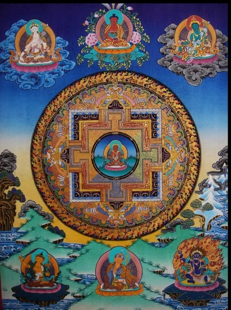
\includegraphics[scale=1]{cosmohindoue.png}
  \hspace{3cm}
  
\includegraphics[scale=1]{genese.png}
  \caption{Gauche : illustration artistique de la cosmologie hindoue. Droite : couverture du livre de la Genèse, Bible de Staint-Paul-hors-des-Murs, vers 870.}
  \label{fig:cosmohindoue}
\end{figure}

Nous pourrions passer la totalité de ce manuscrit à décrire diverses cosmogonies. Mais celle qui nous intéresse et que nous allons détailler ici est la cosmogonie scientifique : la \emph{cosmologie}. La cosmologie est donc l'étude de l'univers, son origine, ses constituants et son devenir, dans le cadre de la méthode scientifique. Même si aujourd'hui la cosmologie fait consensus au sein des scientifiques en ce qui concerne la compréhension de l'univers, cela n'a pas toujours été le cas. Pendant longtemps les croyances religieuses ont dominé, allant jusqu'à limiter voire interdir les avancées scientifiques.
Il faut attendre le \textsc{XVI}\ieme~siècle pour que Copernic propose le modèle héliocentrique, soit presque \num{2000} ans après le modèle géocentrique d'Aristote, soutenu par l'église et les savants jusqu'alors.
% et s'oppose ainsi au modèle géocentrique introduit par d'Aristote et soutenu par l'église et les savants de l'époque.
Par la suite, les observations de Galilée, les travaux de Kepler ainsi que l'émancipation des dogmes religieux ont permis au modèle héliocentrique, fondé sur les lois de Kepler, de s'imposer. Cela a aussi permis à Newton de proposer sa théorie de la gravitation peu de temps après. Cette période marque la naissance de la physique et de la cosmologie.

Jusqu'au \textsc{XIX}\ieme~siècle, le modèle héliocentrique décrivant l'univers comme se limitant à notre système solaire fait consensus. Puis émerge l'idée que les étoiles sont d'autres systèmes solaires, notamment grâce aux premières mesures de distance d'étoiles proches\footnote{Par exemple la mesure de la distance de 61 Cygni par Bessel en 1838. \#prov https://www.universalis.fr/encyclopedie/premiere-determination-de-la-distance-d-une-etoile/.}. L'idée de galaxie, un système rassemblant une multitude de systèmes solaires, fait aussi sont apparition, nous conduisant vers un paradigme de moins en moins anthropocentrique.

\paragraph{}
La cosmologie moderne naît réellement au début du \textsc{XX}\ieme~siècle. En 1915, Einstein propose sa théorie de la gravitation : la \emph{relativité générale}. Elle offre une vision radicalement différente de la théorie bien établie de Newton. La gravitation n'est plus vue comme une force instantannée entre les corps massifs mais comme une déformation de l'espace temps se propageant à la vitesse de la lumière. La théorie d'Einstein prédit correctement l'avance du périhélie de Mercure, dont la valeur était jusque là incomprise. Puis en 1919 lors d'une éclipse de Soleil, la déviation de la lumière par un corps massif, prédiction directe de la relativité générale et non présente dans la théorie de Newton, est observée. Non seulement la déviation de la lumière est observée pour la première fois, mais l'angle de déviation observé correspond à celui prédit par la théorie. Ceci assoit au sein de la communauté scientifique la théorie d'Einstein en tant que nouvelle théorie de la gravitation.

Par ailleurs, la cosmologie observationnelle connaît des avancées remarquables, notamment grâce à Edwin Hubble qui observe le décalage vers le rouge\footnote{voir explication du redshift section~\ref{subsec:descri_mod}, paragraphe \emph{Le redshift}.} du spectre d'objets lointains, dû à leur vitesse d'éloignement. Il comprend aussi que les objets étendus, jusque là interpretés comme des nuages de poussière et de gas et appelés nébuleuses, sont d'autres galaxies semblables à la nôtre. Parallèlement, Alexandre Friedmann résout en 1922 les équations d'Einstein de la relativité générale pour un univers homogène et isotrope et trouve une solution d'univers en expansion, qui contraste avec l'idée d'un univers statique et éternel jusque là ancrée dans les esprits. Enfin, Georges Lemaître effectue le lien entre tous ces éléments. En 1927, il publie un papier explicant que l'éloignement des galaxies et le décalage vers le rouge de leur spectre pouvait être expliqué par une théorie d'univers en expension, et donne la première estimation de la constante de Hubble\footnote{Constante reliant proportionnellement la vitesse d'éloignement des galaxies à leur distance, voir section~\ref{subsec:descri_mod}, paragraphe \emph{Les équations de Friedmann-Lemaître}.}. En 1929, Edwin Hubble publie son célèbre papier, exposant la loi de Hubble et favorisant très fortement le modèle d'univers en expansion.

Nous pouvons noter ici que peu de temps après avoir publié sa théorie, Einstein ajoute dans ses équations une constante ad hoc, dite \emph{constante cosmologique}, et noté $\Lambda$. Cette constante est rajoutée afin de rendre les solutions à ses équations capables de décrire un univers statique (idée dominante de l'époque). Puis, suite à la publication de Hubble, Einstein retire la constante cosmologique de ses équations et la qualifie de ``plus grande bêtise de sa vie''. L'ironie fait qu'en 1998, la constante cosmologique est réintroduite dans les modèles afin d'expliquer l'observation de l'accélération de l'expansion de l'univers (voir \#prov ref). \textbf{Les mesures les plus récentes estiment que la densité d'énergie de cette constante cosmologique, représente environ \SI{70}{\percent} de l'énergie totale de notre univers. La constante cosmologique est parfois appelée \emph{énergie noire}. Ce terme est souvent employé pour désigner les modèles d'accélération d'expansion plus complexes.}

\paragraph{}
Ces quinze années très fertiles pour la cosmologie ont popularisé l'idée d'un univers en expansion. Si certains s'y opposent et défendent un univers statique, d'autres s'y intéressent et étudient en détail les conséquences de ces modèles théoriques. Si l'univers est en expansion, c'est qu'il a été dans le passé plus petit qu'il ne l'est aujourd'hui. L'étude des solutions aux équations d'Einstein montre que l'expansion dilue la matière dans l'univers, et conduit à son refroidissement. L'univers était donc plus chaud et plus dense dans le passé. Si l'on remonte suffisament dans l'histoire de l'univers, celui ci devient de plus en plus petit, jusqu'à n'être à l'origine qu'un point infiniment chaud et dense. Ceci conduit à nommer ces classes de modèles \emph{hot big bang models}, ou modèles de big bang chaud en français. Il est à noter que cet \emph{instant zéro} est une extrapolation des modèles et reste hypothétique : au delà d'une certaine température et densité, les effets quantiques ne peuvent plus être négligés, rendant alors impossible l'utilisation de la relativité générale. Cet instant est appelé mur de Planck. Afin de comprendre ce qu'il se passe entre le mur de Planck et l'instant zéro, une théorie traitant à la fois la gravitation et l'aspect quantique de la matière est nécessaire. C'est un domaine de recherche très dynamique aujourd'hui, dans lequel un grand nombre de théories de gravité quantique sont étudiées.
% . Ces points conduisent à nommer ces classes de solutions \emph{hot big bang models}, ou modèles de big bang en français, symbolisant l'idée qu'à l'origine\footnote{\#prov ou plutôt aussi loin que nous puissions remonter ? Ca vaut peut-être le coup d'expliquer la distinction}, l'univers fût un point infiniment chaud et dense.

Suite notamment aux publications de Friedmann, Lemaître et Hubble, les défenseurs des modèles de big bang ont commencé à chercher des observables capables de prouver ces modèles. En 1948, George Gamow, Ralph Alpher et Robert Herman, reprenant les travaux de Georges Lemaître, prédisent l'existence du \emph{fond diffus cosmologique} (CMB : Cosmic Microwave Background). Ce rayonnement fossile, si les modèles de big bang sont vérifiés, aurait été émis lorsque l'univers était encore dense et chaud. Il repose sur l'idée que, du fait de la température initialement très élevée, les particules possèdent trop d'énergie pour s'assembler et former les premières briques élémentaires. L'univers n'est alors qu'une soupe où toutes les particules s'entrechoquent constamment. Lorsque l'univers s'expand, la température baisse et l'énergie des particules aussi, autorisant ainsi la formation des premiers noyaux d'atomes. Mais la température et la densité sont toujours trop importantes pour laisser les premiers atomes se former : l'univers est alors un bain de noyaux, principalement d'hydrogène et d'hélium, d'électrons et de photons. Les photons sont diffusés constamment sur les électrons libres, rendant le plasma de l'univers primordial opaque. Puis, lorsque l'univers devient suffisamment froid, les électrons ne disposant plus de suffisamment d'énergie sont capturés par les noyaux, formant les premiers atomes de l'univers. Ces atomes, neutres, ne diffusent pas les photons. Ces derniers peuvent alors se propager librement, et l'univers devient transparent. Ce sont ces premiers photons, émis environ \num{380000} ans après le big bang, qui forment le fond diffus cosmologique et que nous pouvons mesurer aujourd'hui. Les principales étapes sont résumées sur la figure~\ref{fig:univershistory}, dont notamment la formation des premiers noyaux vers 0,01 seconde, puis le CMB vers \num{380000} ans.
\textbf{Après l'apparition des premières étoiles, le rayonnement libéré par celles-ci commence progressivement à réionisé l'hydrogène, qui était devenu neutre au moment de l'émission du CMB. Les dernières analyses estiment le redshift de la réionisation à $5 < z_{réionisation} < 9$ (\#prov citer Planck et ?)}
En 1965, 17 ans après sa prédiction, le CMB est détecté par Penzias et Wilson, établissant ainsi le consensus sur les modèles de big bang. A partir de ce moment là, un certain nombre d'observations ont été menées par les cosmologistes afin de contraindre et distinguer les différents modèles de big bang.
\begin{figure}
  \centering
  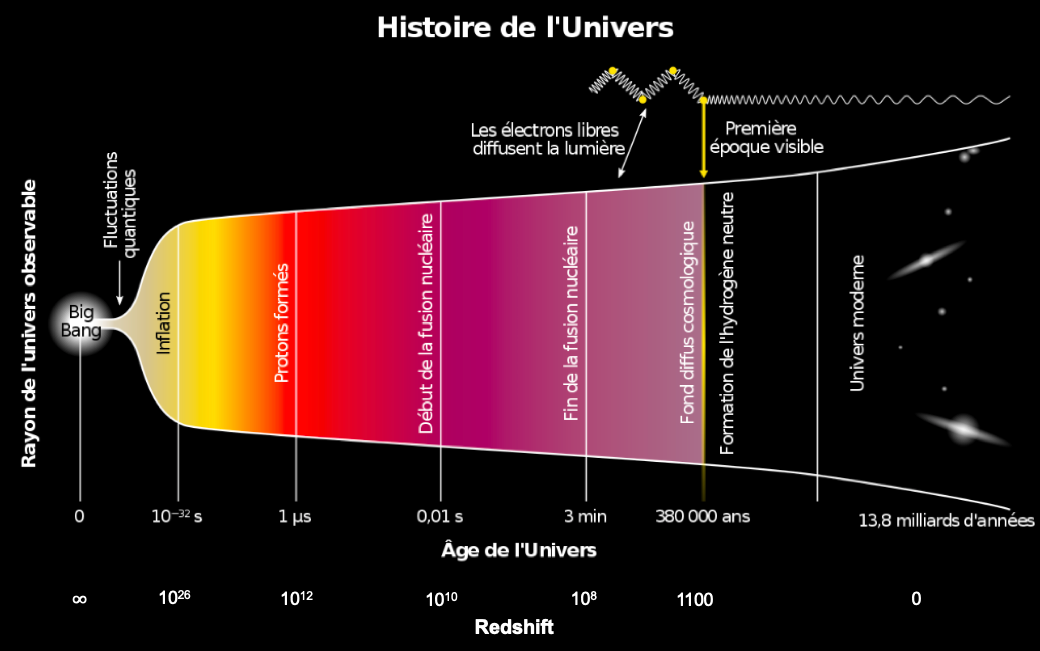
\includegraphics[scale=0.35]{univershistory2}
  \caption{Illustration de l'histoire de l'univers depuis ses origines jusqu'à aujourd'hui. Les principales étapes sont représentées : la formation des premiers protons et neutrons, puis des premiers atomes, et enfin l'emission du CMB.}
  \label{fig:univershistory}
\end{figure}


\section{Le modèle \lcdm{}}

Le modèle \lcdm{} est aujourd'hui le modèle cosmologique qui fait consensus dans la communauté scientifique. Il est souvent désigné comme le modèle standard de la cosmologie. C'est un modèle de big bang, décrivant un univers composé principalement d'énergie noire, ou aussi appelé constante cosmologique ($\Lambda$), et de matière noire froide (CDM : Cold Dark Matter). La figure~\ref{fig:lcdm} présente la répartition de ses différentes composantes.
\begin{figure}
  \centering
  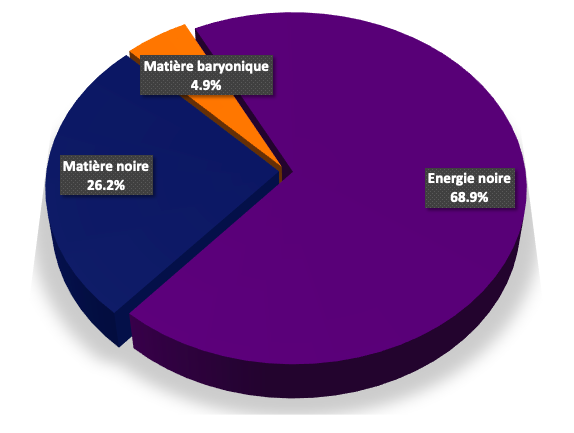
\includegraphics[scale=0.3]{lcdm}
  \caption{Répartition des différentes composantes du modèle \lcdm{}.}
  \label{fig:lcdm}
\end{figure}

Le modèle s'est établi suite à un certain nombre d'observations. D'abord, la détection du CMB en 1965, qui confirme les modèles de big bang.
Puis l'introduction de la matière noire dans les modèles au cours des années 70 et 80, notamment grâce aux travaux de Vera Rubin sur le problème de la masse manquante dans les galaxies. Déja en 1933, Fritz Zwicky remarquait que la masse visible dans les amas n'était pas suffisante pour expliquer leur cohésion, et supposa donc l'existence d'une matière invisible. Une série d'observations fut menée dans les années 70 afin d'étudier les courbes de vitesse des étoiles au sein des galaxies. Les étoiles situées en périphérie furent mesurées avec une vitesse plus importante qu'attendue. La conclusion fut similaire à celle de Zwicky : la présence de masse invisible dans les halos de galaxies permet d'expliquer ces courbes de rotation. Ainsi la matière noire froide fut introduite dans les modèles cosmologiques :
% environ \SI{25}{\percent} de la masse de l'univers est sous la forme d'une matière non standard\footnote{Non-décrite par le modèle standard de la physique des particules.} intéragissant uniquement via la gravitation avec la matière ordinaire.
environ \SI{25}{\percent} de la masse de l'univers est sous la forme d'une matière non standard intéragissant uniquement via la \textbf{gravitation\footnote{Cependant certaines expériences recherchent des particules candidates à la matière noire, qui intéragissent très faiblement via l'intéraction faible, comme par exemple les \emph{WIMPs} (Weakly Interactive Massive Particles)}} avec la matière ordinaire. Nous profitons ici de l'occasion pour présenter le modèle standard de la physique des particules, qui décrit les particules, ainsi que leurs interactions, qui constituent la matière que nous connaissons sur terre. Le modèle standard divise les particules en deux catégories : les bosons et les fermions. Les bosons sont les particules vectrices des interactions. Le photon par exemple, est le boson vecteur de l'interaction électromagnétique. Les fermions quant à eux, constituent la matière. Ils sont classés en deux catégories : les leptons, et les quarks. Les leptons comprennent entre autre les électrons et les neutrinos. Les quarks ne peuvent exister isolément, ils sont regroupés par paires pour former des mésons, ou par trios pour former des baryons. Par exemple, le neutron et le proton sont deux baryons. Les autres baryons ainsi que les mésons sont instables, et possèdent donc une durée de vie courte.
% Ainsi, la matière baryonique désigne la matière formée par l'association de protons et de neutrons, c'est à dire l'ensemble de la matière que nous avons sur terre.
% La matière noire est donc une matière exotique, non décrite par le modèle standard.
\textbf{
  Ainsi, la matière formée par l'association de protons et de neutrons représente l'essentiel de la masse que nous avons sur terre. Cette matière est appelée \emph{matière baryonique}.
La matière noire quand à elle est une matière exotique, non décrite par le modèle standard.
}

% Plus tard, le satelitte COBE fut envoyé dans l'espace afin de mesurer le spectre\footnote{voir explication \#prov:ref} du CMB.
Plus tard, le satellite COBE fut envoyé dans l'espace afin de détecter les anisotropies du CMB. Selon les prédictions des modèles de big bang, le spectre du CMB suit une loi de corps noir, avec une température d'environ \SI{3}{\kelvin}, et possède des anisotropies correspondant aux perturbations primordiales de densité. La mission fut un succès : les mesures de COBE ont permis d'identifier les anisotropies de température du CMB, mettant en évidence les fluctuations de densité de l'univers primordial. D'autre part, le spectre du CMB est mesuré avec une température $T = \SI{2,725(1)}{\kelvin}$ (\#prov Mather et al APJ 1994), ne déviant pas du spectre du corps noir de plus de \SI{0,25}{\percent} \cite{CITE:https://www.ncbi.nlm.nih.gov/pmc/articles/PMC46596/}. La détection des anisotropies du CMB constitue un des arguments les plus solides en faveur des modèles de big bang.

Jusque alors, les modèles cosmologiques n'incluaient pas d'énergie noire. Puis en 1998, deux équipes différentes publient l'analyse de distances de luminosité de supernovae de type 1a (SN1a), toutes les deux mettant en évidence l'accélération de l'expansion de l'univers et donc favorisant les modèles contenant de l'énergie noire. Ce sont ces dernières observations qui ancrent \lcdm{} comme modèle de big bang préféré. Par la suite, le satellites WMAP puis le satellite Planck sont lancés en 2001 et en 2009 afin de mesurer avec une plus grande précision les anisotropies du CMB. Ces mesures successives sont effectuées avec une précision sans précédent, permettant de contraindre très fortement les paramètres cosmologiques. Les résultats finaux de la collaboration Planck ont été publiés en 2018~\cite{CITE:planck2018} et fournissent les paramètres cosmologiques du modèle \lcdm{} avec une précision inférieur au pourcent (voir tableau~\ref{table:planck2018}).

\subsection{Description du modèle}
\label{subsec:descri_mod}

Le modèle \lcdm{}, et plus généralement les modèles de big bang, sont fondés sur le formalisme de la relativité générale.
%\textbf{Cette théorie, élaborée par Einstein en 1915, fait deux postulats. D'abord, elle suppose l'unification de la masse et de l'énergie, via la célèbre formule\footnote{où $E$ est l'énergie, $m$ la masse, et $c$ la vitesse de la lumière dans le vide.} $E = mc²$, ainsi que celle de l'espace et du temps (\#prov check si ce sont vraiment des postulats ou des conséquences, sinon dire juste que ca decoule de relat restreinte + principe equi). Ceci revient à se placer dans le cadre de la relativité restreinte. Elle suppose ensuite le principe d'équivalence}.
Cette théorie, élaborée par Einstein en 1915, est la généralisation de la relativité restreinte, proposée par Einstein 10 ans plus tôt. La relativité restreinte emet deux postulats :
  \begin{itemize}[label=$\bullet$]
  \item les lois de la physique sont les mêmes dans tous les référentiels inertiels\footnote{Un référentiel dans lequel l'observateur n'est pas accéléré.},
  \item la vitesse de la lumière dans le vide est la même dans tous les référentiels inertiels.
  \end{itemize}
Cette théorie traite les mouvements des corps dans les référentiels inertiels, mais n'inclut pas la gravitation. Afin d'inclure la gravitation et d'étendre la théorie aux référentiels accélérés, le principe d'équivalence est supposé.
  % Cette théorie traite donc du mouvements des corps dans des référentiels inertiels. Afin d'étendre la théorie aux référentiels accélérés, et d'ainsi inclure la gravitation, le principe d'équivalence est supposé.  \#correc: c'est plutot generalisation dans le sens ou on inclut la gravitation, et donc les referentiel accelere
Ce principe affirme que la masse inertielle et la masse gravifique sont équivalentes, et que les effets de la gravitation sont identiques aux effets de l'accélération du référentiel de l'observateur. Autrement dit, il n'existe pas d'expérience permettant à l'observateur de distinguer s'il se trouve dans un champ de gravitation uniforme ou dans un référentiel uniformément accéléré. La gravitation n'est alors plus vue comme une force, mais comme un effet géométrique, conséquence de la déformation de l'espace-temps.

Dans la suite de cette section, afin de simplifier les équations, nous nous plaçons dans un système d'unité dans lequel
  \begin{equation}
    c = \hbar = k_{B} = 1 .
  \end{equation}


\paragraph{La métrique —}
Le formalisme de la relativité générale s'appuie donc sur celui de la relativité restreinte. La géométrie de l'espace-temps est décrite par la métrique. Cet objet mathématique\footnote{Un tenseur de rang 2.} permet de définir le produit scalaire sur l'espace-temps à 4 dimensions, et donc de mesurer les distances et les angles.
Nous verrons plus loin dans ce manuscrit que la métrique dépend de la distribution de masse. Ainsi, et c'est le fondement de la relativité générale, la masse courbe l'espace temps et l'espace-temps indique à la masse, via la métrique, comme se déplacer au sein de celui-ci\footnote{Inspiré de la citation de John Wheeler : "Spacetime tells matter how to move; matter tells spacetime how to curve."}. \\
% C'est la métrique qui contient l'information sur la gravitation (\#prov dire que la masse courbe l'espace temps et que c'est traduit par la métrique; voir pour rajouter la citation.
Dans le cadre du modèle \lcdm{}, la métrique utilisée est la métrique FLRW (pour Friedmann Lemaître Robertson Walker), elle s'exprime comme :
\begin{equation}
  \label{eq:metrique1}
  ds² = - dt² + R(t) \left[ \frac{dr²}{1 - k r²} + r² d\Omega \right],
\end{equation}
où $d\Omega = d\theta + \sin(\theta) d\phi$ , $R(t)$ rend compte de l'expansion de l'univers à l'instant $t$, et $k$ vaut soit $1$, $0$ ou $-1$ selon que l'univers possède une courbure positive, nulle ou négative (voir figure~\ref{fig:curvature}).
\begin{figure}
  \centering
  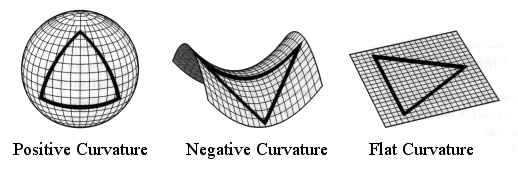
\includegraphics[scale=0.6]{curvature}
  \caption{Représentation de la courbure de l'univers : positive à gauche, négative au centre et nulle à droite.}
  \label{fig:curvature}
\end{figure}
A l'aide d'un changement de coordonnées, il est possible de se ramener à la formule suivante :
\begin{equation}
  \label{eq:metrique2}
  ds² = - dt² + a(t)\left[ d\chi² + S_{k}²(\chi) d\Omega \right],
\end{equation}
où $a(t) = R(t) / R(t₀)$,  $t₀$ est le temps présent et $S_{k}$ est défini comme
\begin{align}
  S_{k}(\chi) = R(t₀) \left\{
    \begin{array}{ll}
      \sin(\chi / R(t₀)) & \mbox{si } k = 1 \\
      \chi / R(t₀) & \textrm{si } k = 0 \\
      \sinh(\chi / R(t₀)) & \mbox{si } k = -1
    \end{array}
\right..
\end{align}
Cette formulation permet de mettre en évidence le rapport $a(t)$, appelé facteur d'échelle. Par définition il vaut 1 aujourd'hui. Afin de rendre compte de l'expansion, $a(t) < 1$ pour $t < t₀$ (passé) et $a(t) > 1$ pour $t > t₀$ (futur).

\paragraph{Le redshift —}
\label{par:redshift}
% Le décalage vers le rouge, ou \emph{redshift} en anglais, est une conséquense de la relativité générale. Les objets distants s'éloignent de nous du fait de l'expansion de l'univers. Similairement à l'effet Doppler\footnote{L'effet Doppler est l'augmentation ou la diminution de la longueur d'onde d'une onde lorsque l'émetteur de cette dernière s'approche ou s'éloigne de l'observateur. L'exemple le plus connu est celui de l'ambulance : le son entendu est plus aigu lorsque l'ambulance s'approche, puis plus grave lorsqu'elle s'éloigne.}, le spectre observé de ces objets est décalé vers les grandes longueurs d'onde. Mais contrairement à l'effet Doppler, le redshift n'est pas directement dû à la vitesse de recession de l'objet : les photons, lorsqu'ils se propagent de l'objet émetteur jusqu'à nous, subissent la dilatation de l'espace et perdent ainsi de l'énergie, leur longueur d'onde se trouvant augmentée \#correction: un peu fishy: demander a Jim sinon. Le redshift est donc du à l'expansion de l'univers. Il est d'ailleurs parfois nommé redshift cosmologique.
% Le redshift, noté $z$, est défini via la relation
% \begin{equation}
%   \label{eq:redshift}
%   1 + z = \frac{\lambda_{o}}{\lambda_{e}},
% \end{equation}
% où $\lambda_{e}$ est la longueur d'onde émise, et $\lambda_{o}$ la longueur d'onde observée. On peut montrer que le reshift est relié au facteur d'échelle via la formule
% \begin{equation}
%   \label{eq:redshift2}
%   1 + z = \frac{1}{a(t)}.
% \end{equation}


Le décalage vers le rouge, ou \emph{redshift} en anglais, est la mesure du décalage du spectre vers les grandes longueurs d'onde des objets distants. Le redshift $z$ est défini comme 
\begin{equation}
  \label{eq:redshift}
  1 + z = \frac{\lambda_o}{\lambda_e} .
\end{equation}
Dans le cadre des modèles de big bang, le redshift est interprété comme une conséquence de l'expansion de l'univers.
Les objets distants s'éloignent de nous du fait de l'expansion. Similairement à l'effet Doppler\footnote{L'effet Doppler est l'augmentation ou la diminution de la longueur d'onde d'une onde lorsque l'émetteur de cette dernière s'approche ou s'éloigne de l'observateur. L'exemple le plus connu est celui de l'ambulance : le son entendu est plus aigu lorsque l'ambulance s'approche, puis plus grave lorsqu'elle s'éloigne.}, le spectre observé de ces objets est décalé vers les grandes longueurs d'onde.
\textbf{
Mais contrairement à l'effet Doppler, le redshift n'est pas directement dû à la vitesse de recession de l'objet :
% les photons, lorsqu'ils se propagent de l'objet émetteur jusqu'à nous, subissent la dilatation de l'espace et voient leur longueur d'onde augmenter. 
% lors de la propagation des photons, l'univers s'expand et ainsi les photons voient leur longueur d'onde augmenter.
à cause de l'expansion, les photons, lors de leur propagation, voient leur longueur d'onde augmenter.
Ceci est dû au facteur d'échelle $a$ présent dans la métrique. En effet, on peut montrer que}
\begin{equation}
  \frac{\lambda_o}{\lambda_e} = \frac{a(t_e)}{a(t_o)} ,
\end{equation}
où $t_e$ et $t_o$ sont les temps d'émission et d'observation du photon, $\lambda_{e}$  et $\lambda_{o}$ sa longueur d'onde lors de l'émission et de l'observation. Le redshift est donc relié au facteur d'échelle via la relation
\begin{equation}
  \label{eq:redshift2}
  1 + z = \frac{1}{a(t)}.
\end{equation} 
Le redshift est donc directement du à l'expansion de l'univers. Il est d'ailleurs parfois nommé redshift cosmologique. Il peut servir de mesure de temps (et aussi de distance, voir section~\ref{subsec:descri_mod} paragraphe \emph{Les distances}) : le spectre d'un objet avec un redshift $z=2$ est décalé vers le rouge d'un facteur 3. Il en découle que sa lumière observée aujourd'hui a été émise lorsque l'univers avait une taille 3 fois plus petite qu'aujourd'hui, soit il y a environ 12 milliards d'annéees.

% (\#correc: en fait on definit le redshift comme le rapport des lambda (c'est independant de la relativite generale), en il se trouve qu'on peut montrer que c'est relie au facteur d'echelle)
% Le décalage vers le rouge, ou \emph{redshift} en anglais, est une conséquense de la relativité générale. Les objets distants s'éloignent de nous du fait de l'expansion de l'univers. Similairement à l'effet Doppler\footnote{L'effet Doppler est l'augmentation ou la diminution de la longueur d'onde d'une onde lorsque l'émetteur de cette dernière s'approche ou s'éloigne de l'observateur. L'exemple le plus connu est celui de l'ambulance : le son entendu est plus aigu lorsque l'ambulance s'approche, puis plus grave lorsqu'elle s'éloigne.}, le spectre observé de ces objets est décalé vers les grandes longueurs d'onde. Mais contrairement à l'effet Doppler, le redshift n'est pas directement dû à la vitesse de recession de l'objet : les photons, lorsqu'ils se propagent de l'objet émetteur jusqu'à nous, subissent la dilatation de l'espace et voient leur longueur d'onde augmenter. Ceci est dû au facteur d'échelle $a$ présent dans la métrique. En effet, on peut montrer que
% \begin{equation}
%   \frac{\lambda_o}{\lambda_e} = \frac{a(t_e)}{a(t_o)} ,
% \end{equation}
% où $t_e$ et $t_o$ sont les temps d'émission et d'observation du photon, $\lambda_{e}$  et $\lambda_{o}$ sa longueur d'onde lors de l'émission et de l'observation.
% % Le redshift est alors définit comme \#prov changer : le redshift est définit comme le raport des lambda et on deduit qu'il est relié à a
% \textbf{Le redshift $z$ mesure alors le décalage vers le rouge d'un objet observé. Il est défini comme
% \begin{equation}
%   \label{eq:redshift}
%   1 + z = \frac{\lambda_o}{\lambda_e} ,
% \end{equation}
% il est relié au facteur d'échelle par
% \begin{equation}
%   \label{eq:redshift2}
%   1 + z = \frac{1}{a(t)}.
% \end{equation} }
% Le redshift est donc directement du à l'expansion de l'univers. Il est d'ailleurs parfois nommé redshift cosmologique. Il peut servir de mesure de temps (et aussi de distance, voir section~\ref{subsec:descri_mod} paragraphe \emph{Les distances}) : le spectre d'un objet avec un redshift $z=2$ est décalé vers le rouge d'un facteur 3. Il en découle que sa lumière observée aujourd'hui a été émise lorsque l'univers avait une taille 3 fois plus petite qu'aujourd'hui, soit il y a environ 12 milliards d'annéees.

% leur longueur d'onde se trouvant augmentée \#correction: un peu fishy: demander a Jim sinon. Le redshift est donc du à l'expansion de l'univers. Il est d'ailleurs parfois nommé redshift cosmologique.
% Le redshift, noté $z$, est défini via la relation
% \begin{equation}
%   \label{eq:redshift}
%   1 + z = \frac{\lambda_{o}}{\lambda_{e}},
% \end{equation}
% où $\lambda_{e}$ est la longueur d'onde émise, et $\lambda_{o}$ la longueur d'onde observée. On peut montrer que le reshift est relié au facteur d'échelle via la formule
% \begin{equation}
%   \label{eq:redshift2}
%   1 + z = \frac{1}{a(t)}.
% \end{equation}

% Ainsi le redshift peut servir de mesure de temps (et aussi de distance, voir distances \#prov) : le spectre d'un objet avec un redshift $z=2$ est décalé vers le rouge d'un facteur 3. Il en découle que sa lumière observé aujourd'hui a été émise lorsque l'univers avait une taille 3 fois plus petite qu'aujourd'hui, soit il y a environ 12 milliards d'annéees.

\paragraph{Les équations d'Einstein —}
Lorsqu'Einstein publie sa théorie en 1915, la façon de présenter les équations d'Einstein, le coeur de la théorie, est différente de la façon de les présenter aujourd'hui. Nous nous proposons ici de suivre l'approche de la physique moderne, qui formule toutes les théories en termes d'un seul et même principe : le \emph{principe de moindre action}. Ce principe stipule que l'action mis en oeuvre lors de l'évolution d'un système entre deux instants est toujours extrémale\footnote{Elle est minimale dans la grande majorité des cas.}. L'action est une quantité caractérisant globalement un système, elle est définie comme
\begin{equation}
  \label{eq:action}
  \mathcal{S} = \int_{t₀}^{t₁} L dt,
\end{equation}
où $L$ est le lagrangien du système. En mécanique newtonienne, il est défini comme la différence de l'énergie cinétique et de l'énergie potentiel. En relativité générale, tout comme dans les théories de champs\footnote{En particulier la théorie quantique des champs.}, le terme du lagrangien est représenté plutôt par une densité de lagrangien. Cette densité de lagrangien est alors intégrée sur l'espace-temps afin d'obtenir l'action. Dans le cas de la relativité générale, l'action est définie comme
\begin{equation}
  \label{eq:actionrg}
  \mathcal{S} = \int d⁴x \sqrt{-g} \frac{R}{4 \pi G} ,
\end{equation}
où $g$ est le déterminant de la métrique, $R$ le scalaire de Ricci, et $G$ la constante de Newton. Le scalaire de Ricci caractérise la courbure, il dépend des dérivées secondes de la métrique. Une fois l'action déterminé, sa minimisation conduit aux équations du mouvement du système. Dans notre cas, ce sont les équations d'Einstein :
\begin{equation}
  \label{eq:einstein}
  R_{\mu \nu} - \frac{1}{2} R g_{\mu \nu} + \Lambda g_{\mu \nu} = 8 \pi G T_{\mu \nu},
\end{equation}
où $g_{\mu \nu}$ est la métrique, $R_{\mu \nu}$ le tenseur de Ricci, $T_{\mu \nu}$ le tenseur énergie-impulsion, et $\Lambda$ la constante cosmologique. Le tenseur de Ricci, dont la contraction donne le scalaire de Ricci $R$, dépend des dérivées secondes de la métrique. C'est donc un terme purement géométrique. Le tenseur énergie-impulsion quant à lui contient l'information de la distribution de masse. Ainsi il y a un lien direct entre la métrique, qui décrit la déformation de l'espace-temps, et la masse présente dans l'univers.

L'équation~\ref{eq:einstein} regroupe en réalité plusieurs équations. Les indices $\mu$ et $\nu$ varient de 0 à 3, 0 représentant la coordonnée temporelle et 1 à 3 les coordonnées spatiales. Il existe donc une équation par couple $(\mu, \nu)$, produisant 16 équations. Par des arguments de symétrie, ce nombre se réduit à 6 équations indépendantes, que l'on nomme les équations d'Einstein.

\paragraph{Les équations de Friedmann-Lemaître —}
Les équations d'Einstein forment un système d'équations différentielles, de second ordre et non linéaires, et de fait, difficile à résoudre. Afin de simplifier les équations et trouver des solutions, certaines hypothèses sont faites. Dans la plupart des modèles cosmologiques, l'univers est supposé homogène et isotrope à grande échelle.
% C'est le cas de la métrique FLRW (voir eq.~\ref{eq:metrique2})
La métrique qui décrit un univers homogène et isotrope est la métrique FLRW (voir l'équation~\ref{eq:metrique2}).
Dans un tel cas, on peut calculer le membre de gauche de l'équation~\ref{eq:einstein}. Ce calcul, que nous ne détaillerons pas ici, est très bien détaillé dans \cite{prov: Dodelson 2.1.2}. De plus, pour un fluide parfait, le tenseur énergie impulsion prend la forme
\begin{equation}
  T_{\mu \nu} =
  \begin{pmatrix}
    -\rho & 0 & 0 & 0 \\
    0 & \mathcal{P} & 0 & 0\\
    0 & 0 & \mathcal{P} & 0\\
    0 & 0 & 0 & \mathcal{P}
  \end{pmatrix} ,
\end{equation}
où $\rho$ est la densité du fluide, et $\mathcal{P}$ est sa pression. Dans ces conditions, la partie temporelle de l'équation~\ref{eq:einstein} donne
\begin{equation}
  \label{eq:friedmann1}
  \left(\frac{\dot{a}}{a}\right)^2 = \frac{8 \pi G}{3}\rho + \frac{\Lambda}{3} - \frac{k}{a^2} 
\end{equation}
et la partie spatiale
\begin{equation}
  \label{eq:friedmann2}
  2 \frac{\ddot{a}}{a} + \left(\frac{\dot{a}}{a}\right)^2 = - 8 \pi G \mathcal{P} + \Lambda - \frac{k}{a^2} ,
\end{equation}
où le point désigne la dérivé temporelle. On définit alors le taux d'expansion $H$ comme $H(t) = \frac{\dot{a}(t)}{a(t)}$. Sa valeur actuelle, notée $H₀$, est appelée constante de Hubble. Elle relie proportionnellement la distance des galaxies à leur vitesse d'éloignement, via la loi de Hubble :
\begin{equation}
  \label{eq:hubble}
  V = H_0 \times D.
\end{equation}
$H_0$ est souvent donné comme $H_{0} = \SI{100}{\h\km\per\s\per\Mpc}$, où $h$ est un paramètre sans dimension qui prend en compte l'incertitude sur $H_0$. D'après les mesures les plus récentes~\cite{CITE planck + Riess ?}, $h$ varie entre $\num{0,67}$ et $\num{0,75}$.
% L'équation~\ref{eq:hubble} est nommée en l'honneur d'Edwin Hubble, après sa publication en 1929, même si Georges Lemaître fut sans doute le premier à saisir le lien entre distance et vitesse d'éloignement des galaxies et son implication concernant l'expansion de l'univers (\#prov a reformuler).
L'équation~\ref{eq:hubble} est nommée en l'honneur d'Edwin Hubble, après sa publication en 1929, même si Georges Lemaître fut sans doute le premier à interpréter le lien entre distance et vitesse d'éloignement des galaxies par l'expansion de l'univers.
Suite à cette brève parenthèse, retournons à nos deux équations. Il est courant de récrire ces équations en injectant $H(t)$, ainsi qu'en remplaçant la seconde par une combinaison linéaire des deux précédentes :
\begin{align}
  \label{eq:friedmann3}
  % \left\{
  %   \begin{array}{l}
  H^2 &= \frac{8 \pi G}{3} \rho + \frac{\Lambda}{3} - \frac{k}{a^2} ,\\
  \label{eq:friedmann4}
        %         - 2 \dot{H} - 3 H^2 = 8 \pi G P + \Lambda + \frac{k}{a^2}
  \frac{\ddot{a}}{a} &= - \frac{4 \pi G}{3} (\rho + 3 \mathcal{P}) + \frac{\Lambda}{3} .
        %       \end{array}
  % \right..
\end{align}
Ces deux équations sont appelées les équations de Friedmann-Lemaître. Elles découlent directement des équations d'Einstein pour un univers homogène et isotrope,
% et permettent de relier les densités d'énergie des différentes composantes de l'univers au facteur d'échelle (\#prov inverser : ca permet d'estimer l'evolution du facteur d'echelle en fonction des compo de l'uni).
et permettent d'estimer l'évolution du facteur d'échelle en fonction des différentes composantes de l'univers.
Nous pouvons noter que le membre de droite de l'équations~\ref{eq:friedmann3} contient 3 entités : le fluide parfait ainsi que la courbure et la constante cosmologique. Même si cela reste un choix d'écriture et ne relève d'aucun argument mathématique, il permet de mettre en évidence le fait que ces deux dernières entités peuvent être considérées comme des composante énergétique de l'univers, avec leur propre densité d'énergie.


\paragraph{Évolution de l'univers —}
Considérons un univers constitué de plusieurs fluides parfaits.
% Les équations de Friedmann-Lemaître permettent de déterminer l'évolution de $\rho$ et $\mathcal{P}$ en fonction du facteur d'échelle. Afin d'obtenir leur évolution temporelle, ainsi que celle du facteur d'échelle, il est nécessaire d'ajouter une équation. Cette équation est l'équation d'état d'un fluide parfait, reliant sa pression à sa densité :
\textbf{Afin de résoudre les équations de Friedmann-Lemaître, et d'obtenir l'évolution de $\rho$ et $\mathcal{P}$ en fonction du facteur d'échelle, il est nécessaire d'ajouter une équation. Cette équation est l'équation d'état d'un fluide parfait, reliant sa pression à sa densité :
\begin{equation}
  \label{eq:etat}
  \mathcal{P} = w \rho,
\end{equation}
où $w$ est le paramètre d'état du fluide, ici supposé constant.
De plus, en utilisant la conservation du tenseur énergie-impulsion $\partial_{\mu} T^{\mu \nu} = 0$, on peut obtenir la relation de conservation pour chaque fluide
\begin{equation}
  \label{eq:conservation}
  \dot{\rho} + 3 H (\rho + \mathcal{P}) = 0 .
\end{equation}
Cette équation peut aussi être obtenue à partir des deux équations de Friedmann-Lemaître. En intégrant cette équation et en utilisant l'équation d'état~\ref{eq:etat}, nous obtenons donc l'évolution de $\rho$ avec le facteur d'échelle}
\begin{equation}
  \label{eq:rho_vs_a}
  \rho = \rho_0 a^{-3(1+w)} ,
\end{equation}
où $\rho_0$ est la densité du fluide considéré aujourd'hui.
Selon le fluide, la valeur de $w$ est différente. Nous pouvons déjà distinguer les particules relativistes\footnote{Une particule est dite relativiste lorsque sa vitesse est proche de celle de la lumière dans le vide.} des particules non relativiste. La matière non relativiste $(m)$ ou simplement matière, se compose de la matière baryonique $(b)$ et de la matière noire froide $(c)$.
\textbf{Elle peut être vue comme un fluide de particules, n'interagissant les unes avec les autres que via la gravitation.} Le fluide correspondant possède alors une pression nulle, son paramètre d'état est donc $w_m = 0$. Nous avons alors : $\rho_m \propto a^{-3}$. \\
Concernant les particules relativistes, elles constituent ce qu'on appelle la radiation $(r)$. La radiation est composée  des photons $(\gamma)$ et des neutrinos relativistes $(\nu)$. Son paramètre d'état est $w_r = 1/3$, ce qui donne $\rho_r \propto a^{-4}$. Nous pouvons remarquer que la densité de matière diminue proportionnellement au volume de l'univers, par simple effet de dilution. La densité de radiation possède un facteur $1/a$ supplémentaire. Ce facteur provient du redshift des photons observés, et s'ajoute au $1/a^3$ de la dilution.

Afin de travailler avec des quantités sans dimension et normalisées, il est courant d'introduire la densité critique $\rho_{crit}$. Cette densité est la densité limite pour laquelle l'univers est plat. Au delà de cette limite, l'univers est fermé, en deçà, l'univers est ouvert. Pour $k = 0$, l'équation~\ref{eq:friedmann3} s'écrit
\begin{equation}
  H^{2} = \frac{8 \pi G }{3} \rho ,
\end{equation}
où $\rho$ désigne la densité totale d'énergie de l'univers, incluant la contribution $\rho_{\Lambda} = \Lambda / 8 \pi G$ de la constante cosmologique, d'où $\rho_{crit} = 3 H_0^2 / 8 \pi G$. En divisant cette équation par $H_{0}^{2}$, l'équation précédente s'écrit alors
\begin{equation}
  \label{eq:friedmann5}
  \frac{H^2}{H_0^2} = \frac{\rho}{\rho_{crit}} .
\end{equation}
A l'aide de l'équation~\ref{eq:rho_vs_a}, chaque composante peut être mise sous la forme
\begin{equation}
  \label{eq:def_omgega}
  \frac{\rho_i}{\rho_{crit}} = \Omega_i a^{-3 (1+w)} , 
\end{equation}
où $\Omega_i$ est le ratio de la densité de l'espèce $i$ par la densité critique aujourd'hui. Nous pouvons alors récrire l'équation de Friedmann-Lemaître~\ref{eq:friedmann3} comme
\begin{equation}
  \label{eq:friedmann6}
  \frac{H^2}{H_0^2} = \sum_i \Omega_i a^{-3 (1+w)} - \frac{k}{a^{2} H_{0}^{2}},
\end{equation}
où $i$ court sur toutes les espèces contribuant à l'énergie totale de l'univers : la matière, la radiation et la constante cosmologique. Ces trois densités relatives valent
\begin{equation}
  \label{eq:def_omega2}
\Omega_{r} = \frac{8 \pi G \rho_{r, 0}}{3 H_{0}^{2}} \hspace{1cm} ; \hspace{1cm} \Omega_{m} = \frac{8 \pi G \rho_{m, 0}}{3 H_{0}^{2}} \hspace{1cm} ;\hspace{1cm} \Omega_{\Lambda} = \frac{\Lambda}{3 H_{0}^{2}} .
\end{equation}
Nous pouvons remarquer ici que $\Omega_{\Lambda}$ est indépendant de $a$. Il en découle $w_{\Lambda} = -1$ : la constante cosmologique peut être interprétée comme un fluide de densité d'énergie constante et de pression négative. Nous verrons par la suite que sa domination dans le bilan énergétique de l'univers actuel est responsable de l'accélération de l'expansion (\#prov voir paragraphe?).
Enfin, en utilisant les définitions précédentes, nous obtenons l'évolution du taux d'expansion
\begin{equation}
  \label{eq:friedmann7}
  H^2 = H_0^2 \left[\Omega_m a^{-3} + \Omega_r a^{-4} + \Omega_{\Lambda} \right] - \frac{k}{a^{2}} .
\end{equation}
% \#prov ca decoule de 1.23 puis 1.24; et peut etre donner omega\_k = 1 - omega\_total Il en découle que pour un univers plat, $\Omega_k = 0$ et donc $\Omega_m + \Omega_r + \Omega_{\Lambda} = 1$.
En évaluant l'équation précédente pour $t=0$, nous obtenons
\begin{equation}
  \label{eq:sum_omega}
 1 + \frac{k}{a^{2} H_{0}}  =  \Omega_m + \Omega_r + \Omega_{\Lambda} = \Omega_{total} .
\end{equation}
Ainsi pour un univers plat, nous avons $k = 0$, et donc $\Omega_{total} = 1$. Nous retrouvons alors que $\rho_{crit}$ correspond à la densité totale de l'univers. 

Bien que les $\Omega_i$ donnent les densités relatives aujourd'hui, nous pouvons comparer les différentes densités d'énergie à n'importe quel redshift, en considérant le rapport $\Omega_{i}(z) = \rho_{i}(z) / \rho_{crit}(z)$, où $\rho_{crit}(z) = 3H(z)^{2} / 8 \pi G$. La figure~\ref{fig:evol_omega} présente l'évolution  avec le redshift des densités relatives, et indique donc les différentes ères de domination. Pour $z > z_{eq}$, c'est la radiation qui domine. Puis vient l'époque de domination de la matière, jusqu'à $z \sim \num{0.3}$. Enfin, c'est la constante cosmologique $\Lambda$ qui domine aujourd'hui.
\begin{figure}
  \centering
  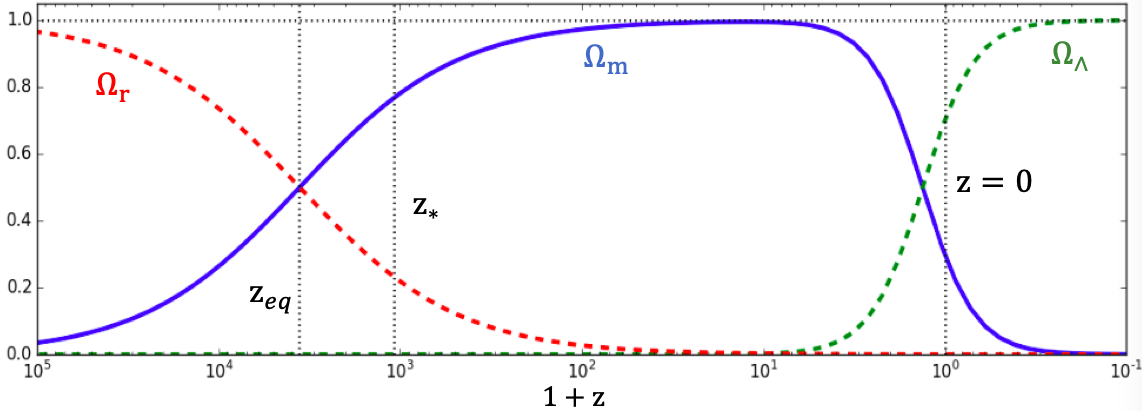
\includegraphics[scale=0.4]{evol_omega}
  \caption{Evolution en fonction du redshift des densités relatives d'énergie pour un univers plat. Sont indiqués en pointillés le redshift d'égalité radiation-matière $z_{eq} = 3387 \pm 21$, le redshift d'émission du CMB $z_{\ast} = \num{1089.80} \pm \num{0.21}$, et le redshift aujourd'hui $z = 0$~\cite{CITEplanck2018}. Crédits : Thèse de Pauline Zarrouk.}
\label{fig:evol_omega}
\end{figure}

Lorsque l'univers est dominé par un seul fluide $i$, nous avons $\rho_{tot} \sim \rho_{i}$, et nous pouvons donc injecter l'équation~\ref{eq:rho_vs_a} dans l'équation de Friedmann-Lemaître~\ref{eq:friedmann3}. Nous obtenons alors l'évolution de taux d'expansion avec le facteur d'échelle
\begin{equation}
  \label{eq:H_evol}
  H = H_0 a^{-3 (1+w) / 2} ,
\end{equation}
ce qui nous donne finalement, pour $w \neq -1$, l'évolution temporelle du facteur d'échelle
\begin{equation}
  \label{eq:a_vs_t}
  a(t) \propto t^{\frac{2}{3(1+w)}} .
\end{equation}
Ainsi, dans chaque phase de domination, $a$ évolue comme une loi de puissance : $a \propto t^{\frac{1}{2}}$ durant l'air de domination de la radiation, puis $a \propto t^{\frac{2}{3}}$ lors de la domination de la matière. Cependant, l'univers est actuellement dominé par l'énergie noire, l'équation différentielle~\ref{eq:H_evol} devient $H = H_0$, et nous obtenons $a \propto \mathrm{e}^{H_{0} t}$. Nous pouvons noter que durant toutes les phases de domination, $\dot a > 0$ : l'univers est en expansion. De plus, lors des phases de domination de la radiation et de la matière, $\ddot a < 0$ : l'expansion de l'univers décélerre. Cependant, pour $ z \lesssim \num{0.3}$, nous avons $\ddot a > 0$, l'univers est alors en expansion accélérée.

% (\#prov Omega\_total prend en compte la courbure ou pas ? C'est pas en accord avec mon equation~\ref{eq:friedmann5}, c'est pas clair ... :\#correc: enlever omega k de omega tot au dessus, c'est plus pedagogique et ne pas le considerer comme une densite d'energie)

% \#prov Il faut peut-etre faire un graph qui montre l'evolution des omega, avec la phase de domination de chaque espèce, et indiquer aussi le z\_eq et z\_CMB etc ; plutot montrer les differentes evolution de a(z) : dans chaque periode de domination on peut calculer comment varie a etc etc. 

% (\#correc : changer la facon de presenter: on considere plusieurs fluides, 1.17, 1.18 et 1.19 sont valables pour chaque fluide separemment; puis plus tard, lors de l'evolution des parametres etc, je peux donner 1.20 et 1.21 quand un seul fluide domine).
% \textbf{Afin de simplifier le raisonnement, nous nous plaçons dans le cas où l'univers est constitué d'un seul fluide parfait. Nous verrons par la suite comment considérer le cas d'un univers composé de plusieurs fluides.
% Pour un fluide donné, les équations de Friedmann-Lemaître permettent de déterminer l'évolution de $\rho$ et $\mathcal{P}$ en fonction du facteur d'échelle. Afin d'obtenir leur évolution temporelle ainsi que celle du facteur d'échelle, il est nécessaire d'ajouter une équation. L'équation généralement choisie (\#correc: pas vraiment le choix enfait) est l'équation d'état d'un fluide parfait, reliant sa pression à sa densité :
% \begin{equation}
%   \label{eq:etat}
%   \mathcal{P} = w \rho,
% \end{equation}
% où $w$ est le paramètre d'état du fluide, ici supposé constant.
% De plus, en utilisant la conservation du tenseur énergie-impulsion $\partial_{\mu} T^{\mu \nu} = 0$, nous obtenons la relation de conservation
% \begin{equation}
%   \label{eq:conservation}
%   \dot{\rho} + 3 H (\rho + \mathcal{P}) = 0 .
% \end{equation}
% En intégrant cette équation et en utilisant l'équation d'état~\ref{eq:etat}, nous obtenons donc l'évolution de $\rho$ avec le facteur d'échelle
% \begin{equation}
%   \label{eq:rho_vs_a}
%   \rho = \rho_0 a^{-3(1+w)} ,
% \end{equation}
% où $\rho_0$ est la densité aujourd'hui. Ainsi, l'évolution de la densité d'énergie de notre fluide dépendra principalement de son paramètre d'état $w$. Si nous injectons maintenant cette équation dans l'équation~\ref{eq:friedmann3}, nous obtenons
% \begin{equation}
%   \label{eq:H_evol}
%   H = H_0 a^{-3 (1+w) / 2} ,
% \end{equation}
% ce qui nous donne finalement
% \begin{equation}
%   \label{eq:a_vs_t}
%   a(t) \propto t^{\frac{2}{3(1+w)}} .
% \end{equation}
% Ce raisonnement est valable pour un univers constitué d'un seul fluide parfait, mais se généralise à un univers contenant plusieurs fluides. }
% Selon le fluide considéré, la valeur de $w$ est différente. Nous pouvons déjà distinguer les particules relativistes des particules non relativiste. La matière non relativiste $(m)$ ou simplement matière, se compose de la matière (\#prov definir baryon etc ici ou avant ? et enlever la note du coup) baryonique\footnote{La matière dite ``ordinaire'', que nous côtoyons dans la vie de tous les jours.} $(b)$ et de la matière noire froide $(c)$.
% % Elle est dite sans pression, donc son paramètre d'état est nul (\#prov expliquer avec les mains : gaz de galaxies qui n'interagissent pas)  : $w_m = 0$. Nous avons alors : $\rho_m \propto a^{-3}$. \\
% \textbf{Elle peut être vue comme un gaz de galaxies, n'interagissant les unes avec les autres que via la gravitation. Le fluide correspondant possède alors une pression nulle, son paramètre d'état est donc $w_m = 0$. Nous avons alors : $\rho_m \propto a^{-3}$. \\}
% Concernant les particules relativistes, qui constituent ce qu'on appelle la radiation $(r)$, elle est composée des photons $(\gamma)$ et des neutrinos relativistes $(\nu)$. Son paramètre d'état est $w_r = 1/3$, ce qui donne $\rho_r \propto a^{-4}$. Nous pouvons remarquer que la densité de matière diminue proportionnellement au volume de l'univers, par simple effet de dilution. La densité de radiation possède un facteur $1/a$ supplémentaire. Ce facteur provient du redshift des photons observés, et s'ajoute au $1/a^3$ de la dilution.
% % dû à l'augmentation de la longueur d'onde des photons avec l'expansion (\#correction fishy, voir avec Jim).
% % Afin de travailler avec des quantités sans dimension et normalisées, il est courant d'introduire la densité critique $\rho_{crit} = 3 H_0^2 / 8 \pi G$ (\#prov expliquer ce que c'est avant de donner la formule). L'équation~\ref{eq:friedmann3} s'écrit alors


% \textbf{Afin de travailler avec des quantités sans dimension et normalisées, il est courant d'introduire la densité critique $\rho_{crit} = 3 H_0^2 / 8 \pi G$. Cette densité correspond à la densité limite pour laquelle l'univers est plat (\#correc: faire reference a l'equation 1.15 et expliquer d'ou ca vient). Au delà de cette limite, l'univers est fermé, en deçà, l'univers est ouvert. En introduisant la densité critique, l'équation~\ref{eq:friedmann3} s'écrit alors}
% \begin{equation}
%   \label{eq:friedmann5}
%   \frac{H^2}{H_0^2} = \frac{\rho}{\rho_{crit}} ,
% \end{equation}
% où $\rho$ représente la densité total d'énergie de l'univers, incluant la contribution de la constante cosmologie $\Lambda$ et de la courbure $k$ (\#correc: expliquer pourquoi on met k dans rho, que c'est un artifice mathematique, donner par exemple rho lambda et rho k, et du coup ptet pas besoin de 1.25 apres). A l'aide de l'équation~\ref{eq:rho_vs_a}, chaque composante peut être mise sous la forme
% \begin{equation}
%   \label{eq:def_omgega}
%   \frac{\rho_i}{\rho_{crit}} = \Omega_i a^{-3 (1+w)} , 
% \end{equation}
% où $\Omega_i$ est le ratio de la densité de l'espèce $i$ par la densité critique aujourd'hui. Nous pouvons alors récrire~\ref{eq:friedmann5} comme
% \begin{equation}
%   \label{eq:friedmann6}
%   \frac{H^2}{H_0^2} = \sum_i \Omega_i a^{-3 (1+w)} ,
% \end{equation}
% où $i$ court sur toutes les espèces contribuant à l'énergie totale de l'univers. Nous avons déjà présenté deux d'entre elles : $\Omega_m$ et $\Omega_r$. Comme mentionné plus tôt, la courbure et la constante cosmologique participent au bilan énergétique global et peuvent être mises sous la forme d'une densité d'énergie, en introduisant
% \begin{equation}
%   \label{eq:omega_lambda}
%   \Omega_{k} = - \frac{k}{a^2 H^2} , \hspace{1cm} \textrm{et} \hspace{1cm} \Omega_{\Lambda} = \frac{\Lambda}{3 H^2} .
% \end{equation}
% Nous pouvons remarquer ici que $\Omega_{\Lambda}$ est indépendant de $a$. Il en découle $w_{\Lambda} = -1$ : la constante cosmologique peut être interprétée comme un fluide de densité d'énergie constante et de pression négative. Nous verrons par la suite que sa domination dans le bilan énergétique de l'univers actuel est responsable de l'accélération de l'expansion (\#prov voir paragraphe?).
% Enfin, en utilisant les deux définitions précédentes, nous obtenons l'évolution du taux d'expansion
% \begin{equation}
%   \label{eq:friedmann7}
%   \frac{H^2}{H_0^2} = \Omega_m a^{-3} + \Omega_r a^{-4} + \Omega_k a^{-2} + \Omega_{\Lambda}.
% \end{equation}
% % \#prov ca decoule de 1.23 puis 1.24; et peut etre donner omega\_k = 1 - omega\_total Il en découle que pour un univers plat, $\Omega_k = 0$ et donc $\Omega_m + \Omega_r + \Omega_{\Lambda} = 1$.
% En évaluant l'équation précédente pour $t=0$, nous obtenons
% \begin{equation}
%   \label{eq:sum_omega}
%  1 - \Omega_k  =  \Omega_m + \Omega_r + \Omega_{\Lambda} = \Omega_{total}
% \end{equation}
% \textbf{Pour un univers plat, nous avons $\Omega_k = 0$, et donc $\Omega_{total} = 1$. Nous retrouvons alors que $\rho_{crit}$ correspond à la densité totale de l'univers. (\#prov Omega\_total prend en compte la courbure ou pas ? C'est pas en accord avec mon equation~\ref{eq:friedmann5}, c'est pas clair ... :\#correc: enlever omega k de omega tot au dessus, c'est plus pedagogique et ne pas le considerer comme une densite d'energie)}

% \#prov Il faut peut-etre faire un graph qui montre l'evolution des omega, avec la phase de domination de chaque espèce, et indiquer aussi le z\_eq et z\_CMB etc ; plutot montrer les differentes evolution de a(z) : dans chaque periode de domination on peut calculer comment varie a etc etc. 

\paragraph{Les distances —}
La notion de distance en relativité générale n'est pas très intuitive.
Du fait de l'expansion, la distance que nous déduisons de l'observation et séparant deux astres lointains n'est pas la distance qui les sépare aujourd'hui. La distance à laquelle nous avons accès est la distance qui séparait ces deux astres lorsque la lumière que nous captons aujourd'hui a été émise. Entre ce moment et aujourd'hui, l'expansion a éloigné ces deux astres et leur distance de séparation a été multipliée par un facteur $\frac{1}{a(t_e)} = 1 + z_{e}$, où $t_e$ est le temps correspondant à l'émission.
Afin de simplifier les comparaisons de distances à différentes époques, nous définissons la distance \emph{comobile} comme ceci : deux objets à un redshift $z$ et séparés d'une distance physique $D$ possèdent une distance comobile $(1+z)D$ . C'est la distance physique telle qu'elle nous apparaîtrait aujourd'hui. Ainsi, la distance comobile séparant deux objets soumis à l'expansion reste la même au cours du temps.
% Du fait de l'expansion, la distance que nous observons entre deux astres lointains n'est pas la distance qui les sépare aujourd'hui. La distance que nous observons est la distance qui séparait ces deux astres lorsque la lumière que nous captons aujourd'hui a été émise. Entre ce moment et aujourd'hui, l'expansion a éloigné ces deux astres et leur distance de séparation a été multipliée par un facteur $\frac{1}{a(t_e)} = 1 + z_{e}$, où $t_e$ est le temps correspondant à l'émission. Afin de simplifier les comparaisons de distances à différentes époques, nous définissons la distance \emph{comobile} comme étant la distance \emph{physique} au moment de l'émission multipliée par $(1+z)$ : c'est la distance physique telle qu'elle nous apparaîtrait aujourd'hui. Ainsi, la distance comobile séparant deux objets soumis à l'expansion reste la même au cours du temps.

Nous présentons ici les différentes distances utilisées en cosmologie. Elles sont très bien décrites dans \cite{CITE: Hogg 1999}, dont nous suivons d'ailleurs les notations. Aussi, nous sortons du cadre dans lequel $c = \hbar = k_{B} = 1$ et nous reprenons le système d'unité usuel. Définissons premièrement la quantité
\begin{equation}
  \label{eq:dist_ez}
  E(z) = \frac{H(z)}{H_0} 
  = \sqrt{\Omega_m a^{-3} + \Omega_r a^{-4} + \Omega_{\Lambda} + 1 - \Omega_{total}} ,
\end{equation}
ainsi que la distance de Hubble aujourd'hui
\begin{equation}
  \label{eq:dist_hubble}
  D_H = \frac{c}{H_0} .
\end{equation}
Nous pouvons alors définir les distances suivantes :
\begin{itemize}[label=$\bullet$]
\item la distance comobile le long de la ligne de visée $D_{C}$. Elle est définie comme
  % comme expliqué précédemment, c'est la distance qui sépare 2 objets suivant le flot de Hubble. Deux objets à un redshift $z$ et séparés d'une distance physique $D$ possèdent une distance comobile $(1+z)D$. La distance comobile le long de la ligne de visé est définie comme
  \begin{equation}
    \label{eq:dist_como}
    D_{C} = D_H \int_0^z \frac{dz'}{E(z')} .
  \end{equation}
\item la distance comobile transverse $D_M$ : deux objets à un redshift $z$ et séparés par un angle $\delta \theta$ sur le ciel possèdent une distance comobile $\delta \theta D_M$.
  Dans le cas où l'univers n'est pas plat ($\Omega_k \neq 0$), la distance comobile transverse $D_M$  n'est pas la même que la distance comobile le long de la ligne de visée $D_{C}$. Elle est reliée à $D_{C}$ par
  \begin{equation}
    \label{eq:dist_como_trans}
    D_M = \left\{
      \begin{array}{ll}
        D_H \frac{1}{\sqrt{\Omega_k}} \sin(\Omega_k D_C / D_H) & \mbox{si } \Omega_k < 0 \\
        D_C & \textrm{si } \Omega_k = 0 \\
        D_H \frac{1}{\sqrt{\Omega_k}} \sinh(\Omega_k D_C / D_H) & \mbox{si } \Omega_k > 0
      \end{array}
    \right..
  \end{equation}
 
\item La distance de diamètre angulaire $D_A$ : c'est la distance reliée à la taille apparente d'un objet. Deux objets à un redshift $z$ et séparés par un angle $\delta \theta$ sur le ciel possèdent une distance physique $\delta \theta D_A$. La distance de diamètre angulaire diffère de $D_M$ du fait qu'elle considère la distance physique et non comobile entre les deux objets. Elle est donc reliée à $D_M$ par
  \begin{equation}
    \label{eq:dist_ang}
    D_A = \frac{D_M}{1+z}.
  \end{equation}

\item la distance de luminosité $D_L$ : elle est définie via la relation qui exprime le flux d'une source lumineuse en fonction de sa luminosité
  \begin{equation}
    \label{eq:dist_lum}
    F = \frac{L}{4\pi D_L²} \hspace{0.5cm} \rightarrow \hspace{0.5cm} D_L = \sqrt{\frac{L}{4 \pi F}} .
  \end{equation}
  Elle est reliée à la distance comobile transverse via
  \begin{equation}
    D_L = (1+z) D_M = (1+z)² D_A ,
  \end{equation}
% \textbf{le facteur (1+z) supplémentaire provenant du fait que les photons sont redshiftés à cause de l'expansion, et perdent donc davantage d'énergie lors de leur propagation jusqu'à nous \#correc: a verifier, peut etre dans le bouquin de Jim. En fait y a un sqrt(1+z) qui vient de lénergie, et sqrt(1+z) qui vient du fait qu'il faut plus de temps aux photons pour cross la sphere de luminosite (p107 dans le bouquin de Jim)}
\end{itemize}

Les distances sont usuellememt mesurées en \si{\perh\kpc} ou \si{\perh\Mpc}, le facteur $\mathrm{h}$ permettant de rendre ces distances indépendantes des erreurs sur la mesure de $H_{0}$. Un parsec vaut environ \num{3.2616} années lumières, soit environ $\SI{3,0857 e16}{\meter}$.
Dans ce manuscrit, les distances qui nous intéressent particulièrement sont $D_C$ et $D_M$. Nous y ferons appel dans la section \#prov ref.

\paragraph{Les paramètres du modèle —} 
Le modèle \lcdm{} est un modèle décrit par 6 paramètres. Ils sont mesurés par le satellite Planck~\cite{CITE ref} avec une précision d'environ 1~\% et sont résumés dans le tableau~\ref{table:planck2018}. Les 6 paramètres mesurés par Planck sont
\begin{itemize}
\item $\Omega_bh^2$, la densité de baryons multipliée par $h^2$
\item $\Omega_ch^2$, la densité de matière noire multipliée par $h^2$
\item $\theta_{MC}$, une approximation de $\theta_*$ : l'angle sur le ciel de l'échelle acoustique
\item $\tau$, la profondeur optique totale, intégrée de $z=0$ jusqu'au CMB. La contribution provient essentiellement des électrons libres entre $z = 0$ et $z_{réionisation}$
\item $A_s$, l'amplitude du spectre de puissance des fluctuations primordiales 
\item $n_s$, l'indice spectrale du spectre de puissance des fluctuations primordiales
\end{itemize}


\begin{table}[h]
  \centering
  \caption{Paramètres cosmologiques mesurés par le satellite Planck. La partie supérieure du tableau indique les six paramètres ajustés aux données. La partie inférieure donne d'autres paramètres déduits de ces six paramètres ajustés. Ces chiffres sont tirés de la table 1.1 de~\ref{CITE ref}}
  \label{table:planck2018}
  \begin{tabular}{lc}
    \toprule
    Parameters & Combined \\
    \midrule
    $\Omega_{\mathrm{b}}h^2$\dotfill & $0.02233\pm0.00015$ \\
    $\Omega_{\mathrm{c}}h^2$\dotfill & $0.1198\pm0.0012$ \\
    $100\theta_{\mathrm{MC}}$\dotfill & $1.04089\pm0.00031$ \\
    $\tau$\dotfill & $0.0540\pm0.0074$ \\
    $\ln(10^{10}A_\mathrm{s})$\dotfill & $3.043\pm0.014$ \\
    $n_\mathrm{s}$\dotfill & $0.9652\pm0.0042$ \\
    \midrule
    $\Omega_{\mathrm{m}} h^2$\dotfill & $ 0.1428\pm 0.0011 $ \\
    $H_0 \,[\si{\kilo\meter\per\second\per\Mpc}]$\dotfill & $67.37\pm0.54$ \\
    $\Omega_{\mathrm{m}}$\dotfill & $0.3147\pm0.0074$ \\
    $\mathrm{Age}\, [\mathrm{Gyr}]$\dotfill  & $13.801\pm0.024$ \\
    $\sigma_8$\dotfill & $0.8101\pm0.0061$ \\
    $S_8\equiv \sigma_8 (\Omega_{\mathrm{m}}/0.3)^{0.5}$\dotfill & $0.830\pm0.013$ \\
    $z_{\mathrm{re}}$\dotfill & $7.64\pm0.74$ \\
    $100\theta_\ast$\dotfill & $1.04108\pm0.00031$ \\
    $r_{\mathrm{drag}} \,[{\rm Mpc}]$\dotfill & $147.18\pm0.29$ \\
    \bottomrule
  \end{tabular}
\end{table}

De ces 6 paramètres se déduisent les autres, notamment les densités d'énergies aujourd'hui, dont nous venons de parler. Certains sont indiqués dans la seconde partie du tableau~\ref{table:planck2018},
dont notamment $r_{drag}$, la taille comobile de l'horizon acoustique au moment du découplage des baryons avec les photons,
ou encore $\Omega_m$ la densité relative de matière aujourd'hui. Les paramètres cosmologiques utilisés pour la confection des simulations présentées dans ce manuscrit et par le code d'analyse \picca{} sont légèrement différents de ceux présentés dans le tableau~\ref{table:planck2018}. Nous les donnons ici :
\begin{equation}
  \label{eq:par_cosmo}
  \Omega_m = \num{0.31457} \hspace{0.5cm} ; \hspace{0.5cm} \Omega_k = \num{0} \hspace{0.5cm} ; \hspace{0.5cm} \Omega_{\Lambda} = \num{0.68543} .
\end{equation}



\section{La fonction de corrélation de la matière}

\textbf{Plus tôt, nous parlions du spectre de puissance des fluctuations primordiales sans avoir auparavant défini ce dont il s'agissait. Nous donnons ici une explication de la notion de spectre de puissance, ainsi que de la fonction de corrélation, objet d'étude de ce manuscrit.}

\subsection{Une analogie avec le son}

\textbf{Prenons l'exemple d'un phénomène simple : le son créé par un diapason. Le diapason est un outil utilisé par les musiciens pour accorder leurs instruments. Lorsqu'il est joué, le diapason produit un signal sonore très proche d'une sinusoïde.}
Le son produit correspond alors à une note particulière, d'une fréquence donnéee, caractéristique de l'instrument. Par opposition au diapason, la corde de guitare par exemple, lorsqu'elle vibre, produit un son composé de plusieurs fréquences : la fréquence fondamentale, qui donne la hauteur de la note, et les fréquences harmoniques, des multiples de la fréquence fondamentale. Ces fréquences harmoniques participent à la richesse du son de l'instrument. L'outil mathématique permettant d'étudier ces phénomènes s'appelle la transformation de Fourier. La transformation de Fourier permet d'associer à un signal temporel, sa transformée de Fourier, un signal dans l'espace des fréquences.

Reprenons l'exemple du diapason. Comme dit précédemment, le signal sonore produit est très proche d'une sinusoïde. La figure~\ref{fig:example_tf} illustre la transformation de Fourier : à gauche se trouve le signal temporel, qui correspond au signal sonore, et à droite se trouve la transformée de Fourier de ce signal.
% Le cas du diapason se situerait plutôt sur la première ligne :
\textbf{La première ligne correspond au cas simplifié du diapason :}
une sinusoïde dont la transformée de Fourier donne un dirac dans l'espace de Fourier, tandis que le cas de la corde de guitare ressemblerait plutôt au cas simplifié de la troisième ligne (\#prov refaire le plot en mettant les harmoniques plutot que des frequences randoms):
une somme de sinusoïdes de différentes fréquences, la fréquence la plus basse donnant la fréquence fondamentale. Dans notre cas, nous pouvons remarquer que le signal dans l'espace fréquentiel est relativement simple : une somme de dirac indiquant les fréquences issues de la décomposition du signal temporel en sinusoïdes.
% il indique la répartition des différentes fréquences présentes dans le signal temporel.
\begin{figure}[h]
  \centering
  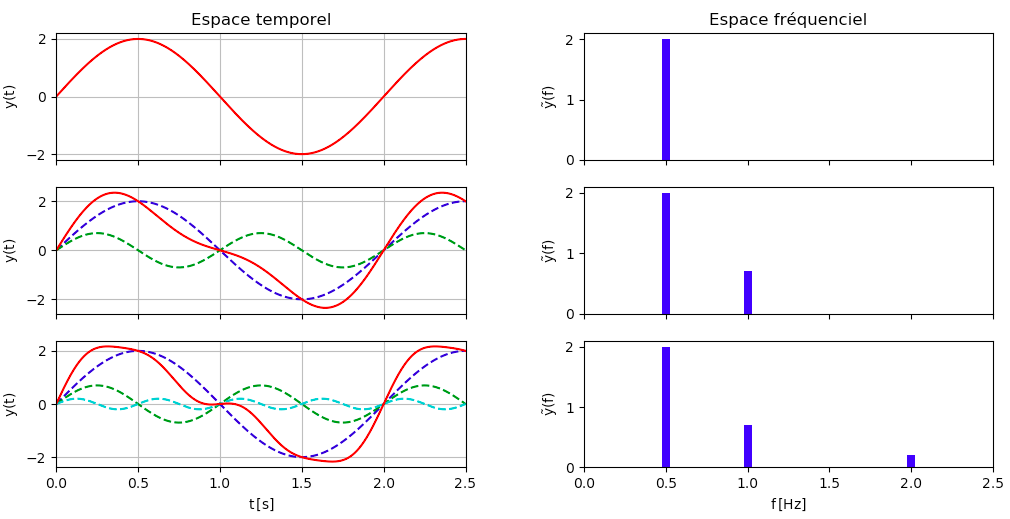
\includegraphics[scale=0.5]{example_tf}
  \caption{Illustration de la transformation de Fourier. Le signal temporel à gauche en rouge est décomposé en somme de sinusoïdes. La transformée de Fourier correspond au signal fréquenciel, à droite, donnant la répartition des fréquences mises en jeu dans le signal temporel.}
  \label{fig:example_tf}
\end{figure}

La transformation de Fourier permet donc de décomposer un signal temporel en une série de sinus et cosinus, et d'indiquer la répartition des différentes fréquences. Pour un signal temporel $f$, la transformée de Fourier $\tilde f$ associée à ce signal est donnée par
\begin{equation}
  \label{eq:def_tf}
  \tilde f(\omega) = \int_{-\infty}^{+\infty}f(t) e^{- i \omega t} dt ,
\end{equation}
où $t$ est le temps en $\si{\second}$, et $\omega$ la pulsation en $\si{\per\second}$. Elle est reliée à la fréquence par $\omega = 2 \pi f$. La transformation inverse est donnée par
\begin{equation}
  \label{eq:def_tf_inv}
   f(t) = \frac{1}{2 \pi}\int_{-\infty}^{+\infty} \tilde f(\omega) e^{ i \omega t} df .
\end{equation}


\subsection{Le spectre de puissance}

\textbf{
  Le spectre de puissance est un outil mathématique utilisé afin d'étudier la répartition des modes présents dans un ensemble de données. Les modes sont la généralisation du concept de fréquence. Par exemple, dans le cas du diapason, les modes sont les différentes fréquences qui composent le signal temporel. En cosmologie, les modes sont associés à des fluctuations spatiales. Prenons l'exemple de la distribution de la matière. On peut définir le contraste de densité en $\vec x$ comme
\begin{equation}
  \label{eq:contraste}
  \delta(\vec x) = \frac{\rho(\vec x) - \bar \rho}{\bar\rho} ,
\end{equation}
où $\rho(\vec x)$ est la densité en $\vec x$, et $\bar \rho$ la densité moyenne. Le spectre de puissance du contraste de densité de la matière renseigne donc sur la répartition des modes de fluctuations spatiales de la matière. La variable dans l'espace de Fourier associée au vecteur position $\vec x$ est le vecteur d'onde $\vec k$. Les grands $k$ correspondent aux modes des petites échelles, et les petits $k$ aux modes des grandes échelles. Le spectre de puissance du contraste de densité de la matière est défini comme
\begin{equation}
  \label{eq:def_pow_spec}
  P(\vec{k}) = \langle \delta(\vec{k'}) \delta(\vec{k}+\vec{k}') \rangle,
\end{equation}
où $\langle.\rangle$ désigne la moyenne sur $\vec{k'}$, et $\delta(\vec{k})$ est le contraste de densité associé au vecteur d'onde $\vec{k}$. Etant donné qu'on suppose l'isotropie en cosmologie, le spectre de puissance dépend uniquement de $k$, la norme de $\vec{k}$. La figure~\#prov montre le spectre de puissance de la matière à $z=0$, elle est discuté dans la section suivante.
}

% Reprenons l'exemple du CMB. (\#prov plutot parler du spectre de puissance de la matiere : presenter le contraste de densite etc). La carte des fluctuations en température est présentée sur la figure~\ref{fig:carte_cmb} et le spectre de puissance associé sur la figure~\ref{fig:spectre_cmb}. 
% \begin{figure}[h]
%   \centering
%   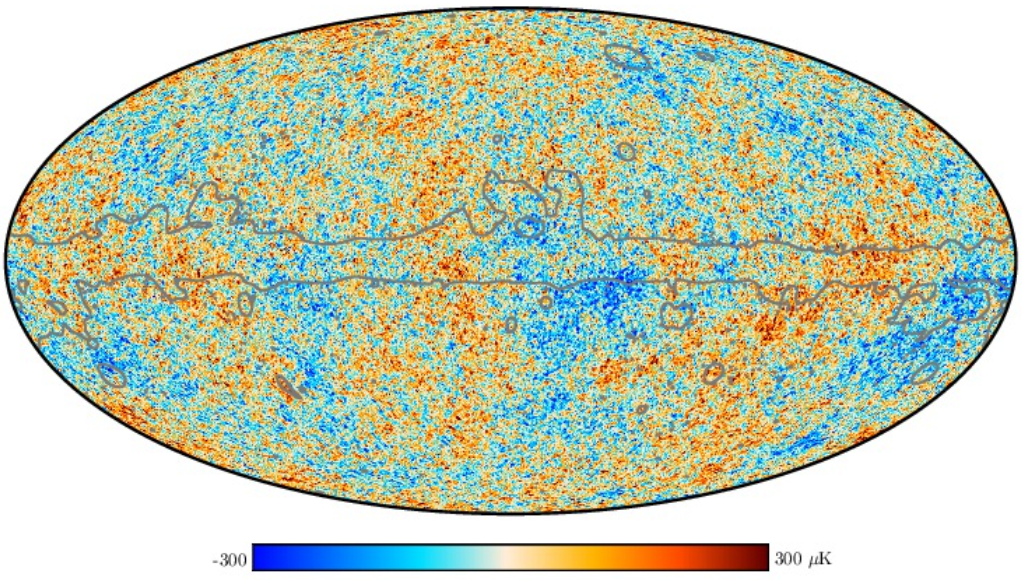
\includegraphics[scale=0.35]{carte_cmb}
%   \caption{Carte des fluctuations en température du CMB. La ligne grise délimite les zones masquées pour éviter la contamination, notamment par la poussière de notre galaxie. Crédits : \cite{CITE:planck2018 legacy}}
%   \label{fig:carte_cmb}
% \end{figure}
% \begin{figure}
%   \centering
%   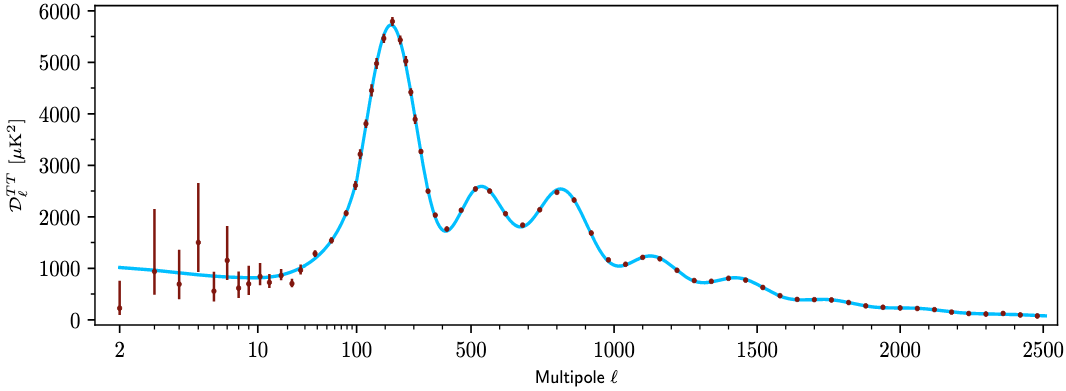
\includegraphics[scale=0.37]{spectre_cmb}
%   \caption{Spectre de puissance des fluctuations en température du CMB. Les points rouges sont les points mesurés, et la ligne bleu indique le meilleur ajustement du modèle \lcdm{}. Crédits : \cite{CITE:planck2018 legacy}}
%   \label{fig:spectre_cmb}
% \end{figure}
% Calculer le spectre de puissance du CMB revient donc à identifier la répartition des modes  dans la carte des fluctuations en température. Le spectre de puissance du CMB présente un pic à $l \sim 200$. Cela signifie que le mode $l \sim 200$ est donc le mode dominant, correspondant à des fluctuations sur le ciel d'une taille caractéristique d'environ $\SI{1}{\degree}$.
% % et que les fluctuations qu'il engendre ont une taille caractéristique d'environ $\SI{1}{\degree}$ sur le ciel.

% Après cette explication imagée de la transformée de Fourier et du spectre du puissance, nous définissons le spectre de puissance comme
% \begin{equation}
%   \label{eq:def_pow_spec}
%   P(\vec{k}) = \langle \delta(\vec{k'}) \delta(\vec{k}+\vec{k}') \rangle,
% \end{equation}
% où $\langle.\rangle$ désigne la moyenne sur $\vec{k'}$, et $\delta(\vec{k})$ est le contraste associé au vecteur d'onde $\vec{k}$. Le contraste est une variable qui renseigne sur l'excès relatif d'une certaine quantité par rapport à la moyenne en chaque point. Par exemple on définit le contraste de densité comme
% \begin{equation}
%   \label{eq:contraste}
%   \delta(\vec{r}) = \frac{\rho(\vec{r}) - \bar \rho}{\bar \rho} ,
% \end{equation}
% où $\rho(\vec{r})$ est la densité en $\vec{r}$ et $\bar \rho$ est la densité moyenne sur tous les $\vec{r}$. Le vecteur d'onde $\vec{k}$ quant à lui est généralement la variable associée dans l'espace de Fourier au vecteur position $\vec{r}$. Etant donné que l'isotropie est supposée en cosmologie, les normes se suffisent à leur vecteur. Ainsi les quantités comme la densité $\rho$ ou le spectre de puissance $P$ ne dépendent que de $r$ ou $k$, la norme des vecteurs $\vec{r}$ et $\vec{k}$.


\subsection{La fonction de corrélation}

% Maintenant que nous avons présenté le spectre de puissance, nous allons décrire la fonction de corrélation, l'objet d'étude de ce manuscrit. Nous nous intéressons particulièrement à la fonction de corrélation de la matière. La distribution de matière dans l'univers peut être vue comme une variable aléatoire 

Maintenant que nous avons présenté le spectre de puissance, nous allons décrire la fonction de corrélation à deux points, l'objet d'étude de ce manuscrit. De la même manière que nous nous sommes intéressés précédemment au spectre de puissance de la matière, nous nous intéressons ici à la fonction de corrélation de la matière. Du fait de l'isotropie de l'univers, cette fonction de corrélation ne dépend que de la distance $r$. Elle permet d'étudier de façon statistique la distribution de matière dans l'univers. Plus exactement, elle donne la corrélation de la distribution de matière entre 2 points de l'espace séparés d'une distance $r$. Similairement au spectre de puissance, la fonction de corrélation du contraste de densité de la matière $\xi$ est définie comme
\begin{equation}
  \label{eq:def_cf}
  \xi(r) = \langle \delta(\vec{r'}) \delta(\vec{r} + \vec{r'}) \rangle,
\end{equation}
où $\langle.\rangle$ désigne la moyenne sur $\vec{r'}$, et $\delta(\vec{r})$ est le contraste de densité.
La fonction de corrélation peut aussi être vue comme un excès de probabilité :
\begin{equation}
  \label{eq:def_cf2}
  dP(r_{1}, r_{2}) = \bar \rho^{2} ( 1 + \xi(r_{1} - r_{2})) dV_{1} dV_{2} ,
\end{equation}
où $dP(r_{1}, r_{2})$ donne la probabilité de trouver de la matière en $r_{1}$ et $r_{2}$.
Ainsi, si la fonction de corrélation $\xi(r)$ est positive, alors il est plus probable de trouver de la matière en deux points de l'espace séparés par une distance $r = r_{1} - r_{2}$ que si celle-ci avait été distribuée de manière uniforme\footnote{Pour une distribution de matière uniforme, $\xi(r) = 0$ pour tout $r$.}.
% Dans le cas de la fonction de corrélation de la matière, $\delta(r)$ est le contraste de densité, comme défini dans l'équation~\ref{eq:contraste}.
On peut montrer que la fonction de corrélation est reliée au spectre de puissance par la transformation de Fourier :
\begin{equation}
  \label{eq:cf_tf}
  P(\vec{k}) = \int \xi(\vec{r}) e^{- i \vec{k} \vec{r}} d^3\vec{r} ,
\end{equation}
ce qui donne, une fois l'isotropie supposée,
\begin{equation}
  \label{eq:cf_tf2}
  P(k) = \frac{i}{4 \pi^2 k} \int_{-\infty}^{+\infty} e^{- i k r} r \xi(r) dr .
\end{equation}
La figure~\ref{CITE} présente le spectre de puissance et~\ref{CITE} la fonction de corrélation de la matière aujourd'hui. (\#prov mettre la figure)
Plusieurs choses sont à noter. Premièrement, le spectre de puissance aux grandes échelles (petits $k$) se comporte comme $P(k) \propto k^{n_s}$, où $n_s$ est l'indice spectrale.
% Ces modes à grande échelle sont directement reliés au spectre de puissance des fluctuations primordiales.
\textbf{Ces modes à grande échelle ne sont pas affectés par la physique qui se déroule durant la domination de la radiation. Ils sondent donc directement les fluctuations primordiales de densité.
Pour les petites échelles (grands $k$), le spectre de puissance est proportionnel à $k^{-3}$. Ce changement de comportement entre les grandes et petites échelles est dû au fait que les modes $k > k_{eq}$, avec  $k_{eq} \sim \SI{0.01}{\h\per\Mpc}$, possèdent une taille caractéristique plus petite que l'horizon\footnote{L'horizon désigne la sphère causale de l'observateur : tout évènemment en dehors de l'horizon n'a pas de lien causal avec l'observateur, car l'information n'a pas eu le temps de se propager jusqu'à ce dernier.} au moment de l'égalité radiation-matière : ces modes sont donc entrés dans l'horizon durant la phase de domination de la radiation, et ont donc été affectés par la physique qui s'y déroule.
% sont entrés dans l'horizon\footnote{L'horizon désigne la sphère causale de l'observateur : tout évènemment en dehors de l'horizon n'a pas de lien causal avec l'observateur, car l'information n'a pas eu le temps de se propager jusqu'à ce dernier.} durant la phase de domination de la radiation : ces modes possèdaient une taille caractéristique plus petite que l'horizon au moment de l'égalité radiation-matière, et ont donc été affectés par la physique qui s'y déroule.
Les modes plus grands que l'horizon au moment de l'égalité radiation-matière ne sont pas affectés par cette physique et sont donc gelés : ils n'évoluent pas, le spectre de puissance reste donc semblable au spectre de puissance primordial.
Les modes plus petits quant à eux sont suppressed (\#prov) durant la phase de domination de la radiation. Plus le mode est petit, plus il entre rapidement dans l'horizon, et plus il est suppressed (\#prov), d'où le changement de comportement pour les $k > k_{eq}$. Après l'égalité, les modes ne sont plus suppressed (\#prov) et tous les modes croissent proportionnellement à $G(z)$. 
$G$ est appelé le facteur de croissance des structures, et varie comme $\mathrm{G}(z) \propto (1+z)^{-1}$ à grand $z$, lorsque $\Omega_m = 1$.} Ainsi, pour des redshifts $z << z_{eq}$, le spectre de puissance varie comme
\begin{equation}
  \label{eq:pow_spec_vs_z}
  P(k,z) = G(z)^{2} P(k,z=0) .
\end{equation}
Le facteur de croissance des structures ne dépendant pas de $k$, la fonction de corrélation est aussi proportionnelle à $G(z)$ :
\begin{equation}
  \label{eq:cf_vs_z}
  \xi(r, z) = G(z)^{2} \xi(r, z=0).
\end{equation}
Tout ceci est un bref résumé de l'évolution des inhomogénéïtés en cosmologie. Cette dernière est très bien décrite dans \ref{CITE:Dodelson chap7} et nous référons le lecteur à cette ouvrage pour davantage d'explications.


Enfin, un point pertinent pour ce manuscrit sont les oscillations présentes dans le spectre de puissance de la matière pour $k \in [\num{0.003} \,; \num{0.3}] \si{\h\per\Mpc}$. Ces oscillations sont dues aux \emph{oscillations acoustiques de baryon} (BAO pour Baryonic Acoustic Oscillations) et sont la trace de la physique qui se déroulait avant l'émission du CMB. Le méchanisme est décrit plus en détail dans la section suivante. Nous pouvons cependant déjà noter que ces oscillations caractéristiques dans le spectre de puissance correspondent au pic présent dans la fonction de corrélation de la matière à $r \sim \SI{100}{\perh\Mpc}$. Ce pic est davantage visible dans le plan $(r, r^{2} \xi(r))$.

\section{Les oscillations acoustiques de baryon}
Les BAO sont une empreinte laissée par la physique pre-recombinaison\footnote{Le moment où les électrons se lient aux protons pour former les premiers atomes.}, et détectable aujourd'hui dans la distribution de matière. Cette empreinte correspond à un excès de corrélation de la matière, à une distance comobile d'environ $\SI{100}{\perh\Mpc}$. Cette distance, appelée \emph{échelle BAO}, fournit une règle standard pour la cosmologie : après l'émission du CMB, la taille comobile de l'échelle BAO reste constante avec le temps.
\textbf{Ainsi, en déduisant l'évolution de la taille physique de l'échelle BAO au cours du temps, grâce notamment à la mesure d'angles et de différences de redshift, nous accédons à l'historique de l'expansion de l'univers.}
% Ainsi, en mesurant l'évolution de la taille physique de l'échelle BAO au cours du temps (\#prov reformuler : on mesure delta z et delta theta), nous accédons à l'historique de l'expansion de l'univers. \\
Dans cette section, nous décrivons les BAO, comment elles se forment, comment elles sont mesurées et les contraintes qu'elles permettent d'établir sur les modèles cosmologiques.

\subsection{La genèse}
Comme expliqué au début de ce manuscrit, l'univers avant la recombinaison est un plasma chaud et dense,
% composé des photons, des baryons, et de la matière noire. L'univers n'étant, initialemment, pas parfaitement homogène,
qui présente de faibles inhomogénéïtés.
% les surdensités présentes produisent des puits de potentiels,
Chaque surdensité produit un puit de potentiel (\#prov c'est vraiment ca qui se passe? a discuter avec Jim),
dans lesquels les particules – les photons, les baryons, la matière noire – tombent.
Les photons et les baryons étant couplés, la pression de radiation augmente au fur et à mesure que la densité augmente. Se joue alors une compétition entre la gravité, qui tend à faire tomber les photons et les baryons dans les puits de potentiel, et la pression de radiation, qui tend à les repousser hors de ce puit de potentiel. Ainsi, les baryons et les photons tombent, puis rebondissent, puis retombent lorsque la pression de radiation devient trop faible, etc.
Ce processus crée donc des oscillations dans le plasma photon-baryon primordial. Comme dans tout milieu, ces oscillations donnent lieu à des ondes acoustiques, qui se propagent à la vitesse du son dans ce milieu. Celle-ci s'exprime comme
\begin{equation}
  \label{eq:sound_speed}
  c_{s} = \sqrt{\frac{1}{3(1 + R)}},
\end{equation}
où $R = \frac{3\rho_b}{4\rho_{\gamma}}$. Etant donné que la densité de photons $\rho_{\gamma}$ est bien suppérieure à la densité de baryons $\rho_{b}$, la vitesse du son $c_s$ vaut $1/\sqrt{3}$ en bonne approximation.
\begin{figure}
  \centering
  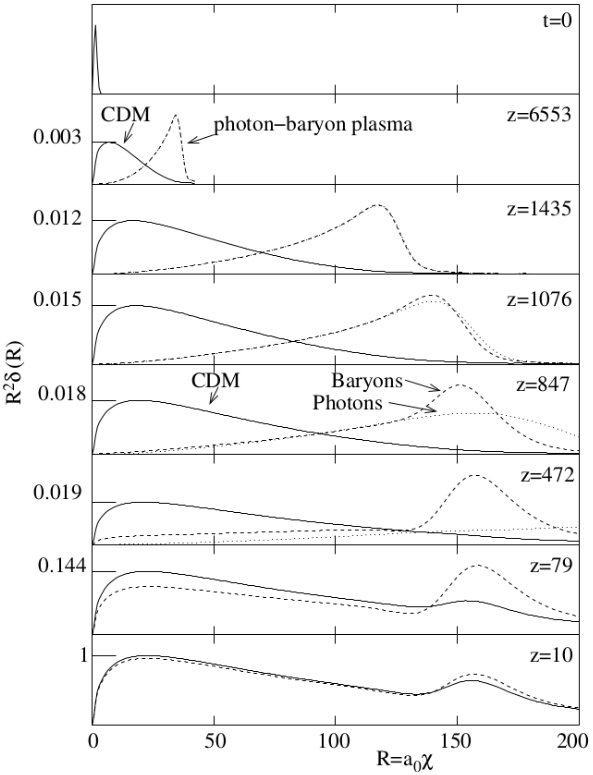
\includegraphics[scale=0.5]{bao_schema}
  \caption{bla}
  \label{fig:bao_schema}
\end{figure}
Ces ondes acoustiques se propagent donc dans le plasma primordial depuis chaque surdensité . La figure~\ref{fig:bao_schema} schématise le méchanisme pour une seule surdensité. A l'instant $t=0$, nous considérons donc une surdensité en $R = \SI{0}{\Mpc}$. Cette surdensité est composée de matière noire (CDM), de baryons et de photons. Le puit de potentiel créé fait s'effondrer (\#prov : a discuter) les espèces présentes, jusqu'à ce que la pression de radiation devienne suffisante pour initier une onde acoustique. Au fur et à mesure que le temps s'écoule (le redshift diminue), le front d'onde dans le plasma photon-baryon se propage. \textbf{Puis, à un redshift $z_{drag} \sim 1060$, les baryons se découplent des photons. La pression dans le milieu devient nulle, faisant chuter la vitesse du son à zéro. L'onde est alors gelée.} Ainsi la surdensité de baryon ne se propage plus, et les photons, qui n'interagissent plus avec les baryons, se propagent librement. La surdensité de matière noire à $R = 0$, qui a continué de croître, rappelle les baryons par effet gravitationnel. Cependant, la surdensité de baryon à $R \sim \SI{150}{\Mpc}$ produit aussi un puit de potentiel, dans lequel la matière noire alentour tombe progressivement. Ainsi, même si la majeure partie des baryons retombent dans le puit de potentiel créé par la surdensité initiale, un second puit de potentiel, formé par des baryons et de la matière noire, subsiste en $R \sim \SI{150}{\Mpc}$. Nous pouvons généraliser cette vue simplifiée en une dimension à 3 dimensions : le front d'onde qui se propagent à partir de la surdensité initiale est alors sphérique, et le second puit de potentiel résultant est alors une sphère centrée sur la surdensité initiale et de rayon $R \sim \SI{150}{\Mpc}$. Cette distance d'environ $\SI{150}{\Mpc}$ est appelée \emph{horizon acoustique} : c'est la distance que l'onde sonore a pu parcourir avant d'être gelée. L'horizon acoustique est défini comme
\begin{equation}
  \label{eq:sound_horizon}
  r_{d} = \int^{\infty}_{z_{drag}} \frac{c_{s}}{H(z)} dz ,
\end{equation}
et vaut $r_{d} = \SI{99.16(20)}{\perh\Mpc}$ selon~\ref{CITE planck2018}.

Ce processus a laissé des traces dans la distribution de matière à grande échelle : à chaque surdensité primordiale est associée une sphère de surdensité de rayon comobile $\SI{150}{\Mpc}$. Ainsi, lorsque nous observons aujourd'hui un traceur de la densité de matière, telle une galaxie, il est davantage probable d'en trouver d'autres, séparés du premier d'une distance comobile d'environ $\SI{150}{\Mpc}$. C'est ce que traduit le pic BAO présent dans la fonction de corrélation de la matière, montrée sur la figure~\ref{fig:CITE figure CF}


\subsection{Mesurer l'échelle BAO}

Comme nous allons le voir dans ce qui suit, les analyses BAO ne mesurent pas directement l'échelle BAO, $r_{d}$. En cosmologie, les observations  ne permettent pas de mesurer des distances. Les informations auxquelles l'observateur a accès sont des différences de vitesse le long de la ligne de visé, via l'observation des spectres, ainsi que des angles, via les projections sur la sphère céleste.
%Afin d'expliquer les mesures des analyses BAO, nous supposons un cas simplifié en deux dimensions, où l'observateur identifie une surdensité primordiale et l'horizon acoustique qui lui correspond, via l'observation de galaxies. Le schéma~\ref{fig:bao_dessin} illustre la situation.
\textbf{Afin d'expliquer les mesures des analyses BAO, nous considérons la situation du schéma~\ref{fig:bao_dessin}, où l'observateur identifie une surdensité primordiale et l'horizon acoustique qui lui correspond, via l'observation de galaxies.}
\begin{figure}
  \centering
  \label{fig:bao_dessin}
  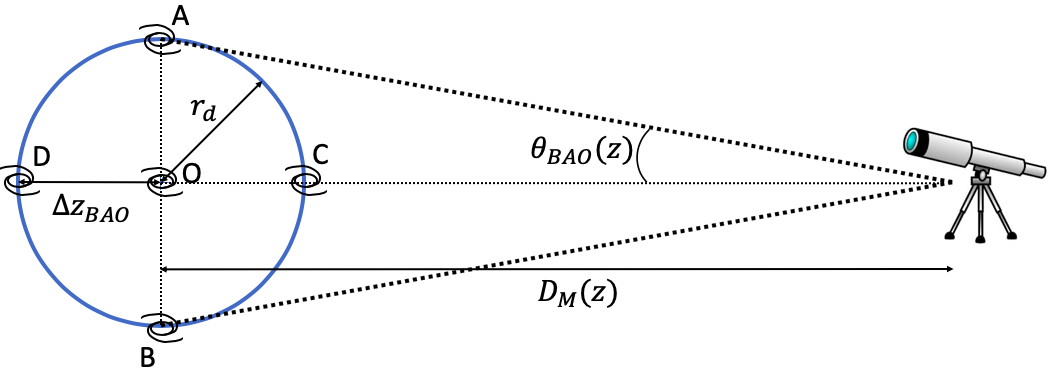
\includegraphics[scale=0.40]{bao_dessin}
  \caption{bla}
\end{figure}
Le cercle bleu représente l'horizon acoustique, et le point $\mathcal{O}$ la surdensité promordiale. Grâce aux galaxies situées en $\mathcal{O}$ , $\mathcal{A}$  et $\mathcal{D}$, l'observateur a accès à deux informations : l'angle $\theta_{BAO}(z)$ séparant $\mathcal{O}$ et $\mathcal{A}$, et la différence de redshift $\Delta z_{BAO}$ entre $\mathcal{O}$ et $\mathcal{D}$. Comme décrit dans le paragraphe sur les distances, l'angle $\theta_{BAO}(z)$ est relié à la distance comobile transverse $D_M(z)$ par
\begin{equation}
  \label{eq:theta_bao}
  \theta_{BAO}(z) = \frac{r_d}{D_M(z)}.
\end{equation}
Ainsi, dans la direction transverse à la direction d'observation, l'observateur mesure le rapport $D_M(z) / r_d$. Le long de la ligne de visée, l'observateur peut comparer les spectres des galaxies en $\mathcal{O}$ et en $\mathcal{D}$, et déduire la différence de redshift $\Delta z_{BAO}$ qui existe entre les deux, due à la distance $r_d$ qui les sépare. La différence de redshift est proportionnelle à la différence de vitesse $\Delta v_{BAO}(z)$, qui s'exprime grâce à la loi de Hubble comme
\begin{equation}
  \label{eq:v_bao}
\Delta z = \frac{\Delta v_{BAO}(z)}{c} =   \frac{\Delta v_{BAO}(z)}{c} = \frac{H(z) r_d}{c} ,
\end{equation}
et est donc reliée à la distance de Hubble $D_H(z)$ par :
\begin{equation}
  \label{eq:v_bao2}
  \Delta v_{BAO}(z) = \frac{r_d }{D_H(z)}.
\end{equation}
Les deux informations accessibles et pertinentes pour les analyses BAO sont donc les quantités $D_M(z) / r_d$ et $D_H(z) / r_d$. Comme dans beaucoup d'analyses cosmologiques, les analyses BAO nécessitent de supposer une cosmologie, afin notamment de transformer les angles et différences de redshift en distance. Ces analyses ne mesurent alors pas directement les rapports  $D_M(z) / r_d$ et $D_H(z) / r_d$ mais leur déviation par rapport à la cosmologie de référence utilisée dans l'analyse, que l'on nomme \emph{cosmologie fiducielle}. Il est donc coutume de définir les quantités $\apar{}$ et $\aperp{}$ comme
\begin{align}
  \label{eq:apar}
  \apar{}(z) &= \frac{D_H(z) / r_d}{(D_H(z) / r_d)_{fiducielle}} , \\
  \label{eq:aperp}
  \aperp{}(z) &= \frac{D_M(z) / r_d}{(D_M(z) / r_d)_{fiducielle}} ,
\end{align}
qui valent $1$ si la cosmologie observée et la même que la cosmologie fiducielle.


\subsection{Contraintes cosmologiques}
Indépendamment d'autres sondes cosmologiques, telles le CMB ou les supernovae, les BAO permettent de mesurer les rapports $D_M(z) / r_d$ et $D_H(z) / r_d$. Ces rapports sont reliés aux paramètres cosmologiques par
\begin{align}
  D_H(z) / r_d &= \frac{1}{H_0 E(z) r_d}, \\
  D_M(z) / r_d &= \frac{1}{H_0 E(z) r_d} \int_0^z \frac{dz'}{E(z')},
\end{align}
où $E(z) = \sqrt{\Omega_m (1+z)^3 + \Omega_{\Lambda} + 1 - \Omega_{total}}$, pour des redshifts bien inférieurs à $z_{eq}$. \\
Ainsi, sans faire de supposition sur le modèle cosmologique, comme par exemple la platitude, les BAO permettent de contraindre les paramètres $(\Omega_{m} , \Omega_{\Lambda} , H_0 r_d)$ du modèle (o)\lcdm{}.
\#prov rajouter autre chose ? Montrer un plot omega m / omega lambda ?
Mettre un plot qui montre H(z) / (1+z) (deceleration puis acceleration etc etc)

\section{Traceurs de la matière}
Jusqu'à maintenant, nous avons beaucoup mentionné la fonction de corrélation et le spectre de puissance de la matière. Pourtant, c'est quelque chose qui en pratique n'est pas accessible. En effet, la matière est constituée à \SI{85}{\percent} de matière noire qui, par définition, n'est pas visible. La seule matière observable est la matière baryonique, via l'observation de traceurs. Du fait de la nature de ces traceurs, le champ de matière sondé diffère du champ de matière total sous-jacent, et par conséquent, la fonction de corrélation obtenue à l'aide de ces traceurs n'est pas la fonction de corrélation de la matière. Dans cette section, nous décrivons les différents traceurs utilisés dans l'analyse présentée dans ce manuscrit, et comment, à l'aide de leur fonction de corrélation, déduire la fonction de corrélation de la matière.
% Bien sûr, la matière baryonique suit sensiblement la même distribution que celle de la matière noire, mais des différences subsistent et leur fonction de corrélation diffèrent. Dans cette section, nous décrivons les différentes façons de sonder la distribution de matière baryonique, et comment déduire la fonction de corrélation de la matière à partir de celle-là.


\subsection{Traceur et biais}
Le moyen le plus évident auquel nous pouvons penser pour sonder la matière est l'observation de la matière baryonique via la lumière qu'elle émet. Les étoiles en sont un bon exemple. La lumière qu'elles émettent nous permet de les localiser dans notre galaxies, à la différence des planètes qui sont quasiment invisibles. C'est notamnent grâce à la lumière émise par les milliards l'étoiles présentes dans les galaxies que nous pouvons observer ces dernières. Mais ceci présente un défaut : la distribution que tracent les étoiles ou les galaxies n'est pas la distribution de matière sous-jacente.

Prenons un exemple. Supposons que nous voulons reconstruire la distribution de la matière dans une région de l'espace. Pour ce faire, nous observons toutes les galaxies, que nous supposons identiques, dans cette région. La figure~\ref{fig:schema_biais} schématise la distribution de ces galaxies, ainsi que la distribution de la matière sous-jacente.
\begin{figure}
  \centering
  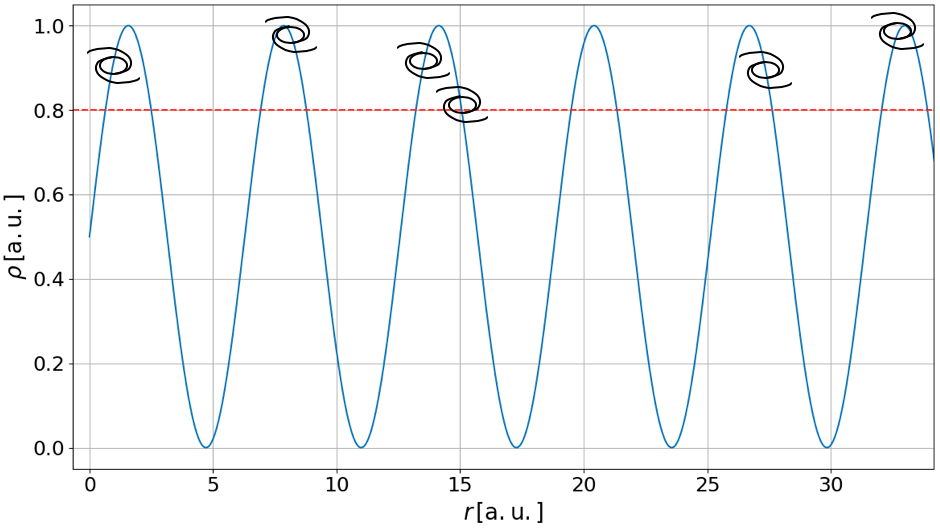
\includegraphics[scale=0.4]{schema_biais}
  \caption{blabla}
  \label{fig:schema_biais}
\end{figure}
Les galaxies, comme tous les objets effondrés, se forment dans les endroits les plus denses de l'univers. Ceci est illustré sur la figure~\ref{fig:schema_biais} par le fait que les galaxies ne peuvent se former que pour des densitées $\rho > \num{0.8}$. Ainsi, sonder la distribution de matière via l'observation des galaxies nous fait manquer toute la distribution de matière pour laquelle $\rho < \num{0.8}$. La distribution reconstruite sera donc plus clustered (\#prov) que la distribution sous-jacente. Ce phénomène est décrit par ce qu'on nomme le \emph{biais}. Le biais $b_i(z)$ du traceur $i$ au redshift $z$ est défini par
\begin{equation}
  \label{eq:biais1}
  \delta_{i}(\vec r, z) = b_{i}(z) \delta_{matière}(\vec r, z), 
\end{equation}
où $\delta_{i}$ est le contraste de densité relatif au traceur $i$, et $\delta_{matière}$ le contraste de densité de la distribution de matière sous-jacente. Le biais relie donc les fluctuations de densités relatives au traceur $i$, aux fluctuations de densités de la matière. Pour les objets compacts, telles les galaxies, le biais est supérieur à 1. Plus le traceur se forme dans des régions denses, et plus le biais est grand. Ainsi, grâce à la relation précédente, nous pouvons relier la fonction de corrélation du traceur $i$ à celle de la matière par
\begin{equation}
  \label{eq:biais2}
  \xi_{i}(r, z) = b_{i}^2(z) \xi_{matière}(r, z) .
\end{equation}
La fonction de corrélation associée au traceur $i$ est amplifiée par un facteur $b_{i}^2$. Il est donc avantageux de choisir un traceur avec un biais important, afin d'obtenir une fonction de corrélation avec une amplitude importante, et ainsi un rapport signal sur bruit plus grand.

\subsection{Distorsions dans l'espace des redshifts}
Afin de construire la fonction de corrélation du traceur $i$, il est nécessaire de connaître le redshift de chaque traceur. Dans le cas des traceurs booléens, comme par exemple les galaxies, le redshift est obtenu en mesurant le spectre de l'objet, puis en comparant les longueurs d'onde des raies d'émission présentes dans le spectre aux longueurs d'onde mesurées en laboratoire. Le redshift mesuré est donc le suivant :
\begin{equation}
  z_{mesure} = z_{vrai} + \Delta z_{v} + \delta z_{sys} + \delta z_{stat} ,
\end{equation}
où $z_{mesure}$ est le redshift mesuré, $\delta z_{sys}$ et $\delta z_{stat}$ sont les erreurs statistiques et systématiques sur la mesure du redshift, $z_{vrai}$ est le vrai redshift, inaccessible, et $\Delta z_{v}$ et le redshift induit par la vitesse particulière du traceur. En effet, en plus du redshift cosmologique, l'effet Doppler vient s'ajouter à la mesure du redshift. Ces deux effets sont indiscernables. Cependant, la vitesse particulière du traceur est corrélée avec le champ de matière sous-jacent : les traceurs ont tendance à se déplacer vers les surdensités, par effet gravitationnel. La figure~\ref{fig:schema_rsd} illustre la situation : au centre se trouve une surdensité, représentée par un amas de galaxies. Quatre galaxies se trouvent autour de cette surdensité, leur vitesse particulière est représentée par une flèche noire, qui est dirigée vers le centre à cause du puit de potentiel créé par la surdensité. La galaxie se trouvant derrière cette surdensité se déplace donc vers l'observateur, son redshift mesuré est ainsi plus petit que son redshift cosmologique. Similairement, la galaxie se trouvant devant la surdensité est reconstuire avec une redshift plus grand. Les objets se déplaçant perpendiculairement à la ligne de visée ne sont pas affectés. La ligne en pointillés bleu indique la distribution reconstruite dans l'espace des redshifts : cette distribution n'est plus circulaire, elle est aplatie selon la direction de la ligne de visée. Cette effet est appelé \emph{RSD} (Redshift Space Distorsions), ou \emph{distorsions dans l'espace des redshifts}.
\begin{figure}
  \centering
  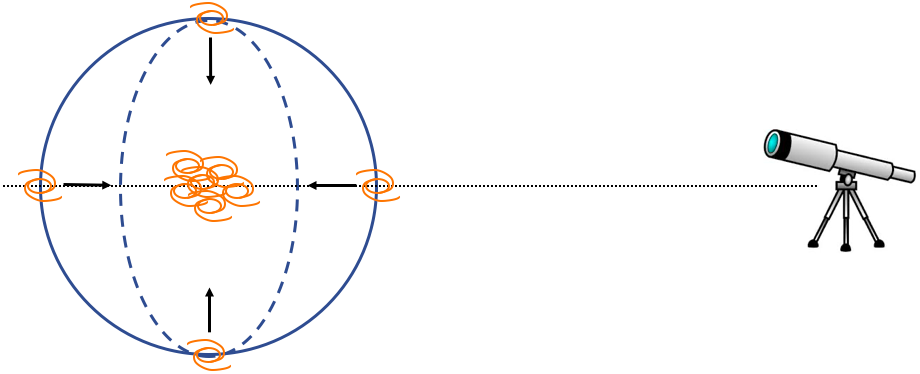
\includegraphics[scale=0.4]{schema_rsd}
  \caption{bla}
  \label{fig:schema_rsd}
\end{figure}

Ces distorsions résultent d'un effet gravitationnel : les traceurs acquièrent leur vitesse en tombant dans les puits de potentiel créés par les surdensités. L'effet peut donc être modélisé. La formule de Kaiser~\cite{CITE} relie le contraste de densité $\delta^s(\vec k)$ dans l'espace des redshifts au contraste de densité $\delta(\vec k)$ dans l'espace réel
\begin{equation}
  \label{eq:kaiser}
  \delta^{s}(\vec k, z) = (1 + f(z) \mu^2) \delta(\vec k, z) ,
\end{equation}
où $f = \frac{d \ln{G}}{d \ln{a}}$ est le taux de croissance logarithmique, et $\mu = \frac{\vec k \cdot \vec u}{k}$, où $\vec u$ est la direction de la ligne de visée. Lorsque le champ de matière est sondé dans l'espace des redshifts à l'aide d'un traceur $i$, l'équation précédente devient
\begin{equation}
  \label{eq:kaiser2}
  \delta_i^{s}(\vec k, z) = (b_i(z) + f(z) \mu^2) \delta_{matière}(\vec k, z) .
\end{equation}
De cette équation, nous déduisons la relation entre la fonction de corrélation $\xi_{i}^{s}$ du traceur $i$ dans l'espace des redshifts et la fonction de corrélation de la matière :
\begin{equation}
  \label{eq:kaiser3}
  \xi_{i}^s(r, \mu, z) = b_{i}^2(z)(1 + \beta_i(z) \mu^2)^2 \xi_{matière}(r, z) ,
\end{equation}
où $\beta_i = f / b_i$ est le paramètre RSD du traceur $i$, et $\mu =\frac{\vec r \cdot \vec u}{r}$. Le vecteur $\vec r$ peut être décomposé comme $\vec r = \rpar{} \vec u + \vec \rperp{}$, où $\vec \rperp{}$ est perpendiculaire à la ligne de visée. La quantité $\mu$ vaut alors $\rpar{} / r$. Du fait de l'isotropie dans la direction transverse à la ligne de visée, $\xi_i^s$ ne dépend que de la norme de $\vec \rperp{}$.

L'analyse de la fonction de corrélation selon $\rpar{}$ et $\rperp{}$ permet donc non seulement de mener une analyse BAO : mesurer la position du pic afin de déduire les quantités $D_{H} / r_d$ et $D_{M} / r_d$, mais aussi de mener une analyse dite RSD : mesurer $\xi_i^s(\rpar{}, \rperp{})$ afin de déduire $b_i$ et $\beta_i$ et ainsi mesurer $f$. Le taux de croissance logarithmique $f$ est une prédiction de la relativité générale, pour un univers dominé par la matière, il vaut $f = \Omega_{m}^{\num{0.55}}$. La mesure de $f$ est donc un test direct de la relativité générale. (\#prov nécessite une source ? Besoin de détailler plus les analyses RSD ? Parler de sigma8 ?)

\subsection{Les quasars}
Les quasars, pour \emph{quasi - star}, sont les objets les plus lumineux de l'univers. Ils font parties des galaxies actives, abrégées AGN (\emph{Active galatic nuclei}). Ces galaxies hébergent en leur centre un trou noir supermassif, de quelques millions à plusieurs milliards de masses solaires. La figure~\ref{fig:schema_qso} schématise le noyau actif. 
\begin{figure}
  \centering
  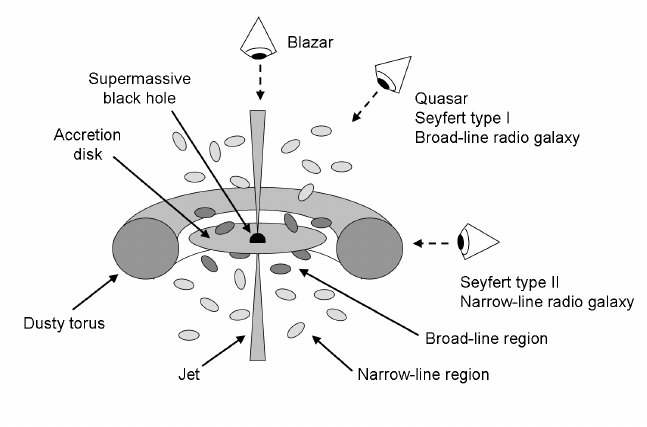
\includegraphics[scale=0.5]{schema_qso.png}
  \caption{bla}
  \label{fig:schema_qso}
\end{figure}
Le trou noir supermassif, au centre, acrète la matière environnante. Sous forme d'un disque, cette dernière s'échauffe en tombant et rayonne énormément d'énergie, dans toutes les longueurs d'ondes. Selon les cas, et souvent par cycle, le noyau actif peut émettre de puissants jets de matière ultra-relativiste. La figure~\ref{fig:qso_jets} montre de tels jets. Ces jets, d'une taille de plus de \SI{200}{\perh\kpc}, sont principalement constitués de noyaux ionisés, d'électron et de positrons, éjectés à une vitesse proche de celle de la lumière. Ces phénomènes font partis des plus énergétiques de l'univers.
\begin{figure}
  \centering
  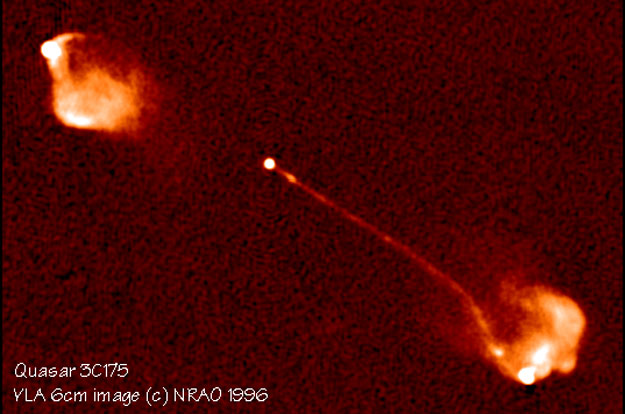
\includegraphics[scale=0.4]{qso_jets}
  \caption{Image radio du quasar 3C 175 prise avec le VLA. Les deux jets ultra-relativistes visibles ont une taille d'environ \SI{212}{\perh\kpc}. Crédits : \cite{CITE http://adsabs.harvard.edu/full/1994AJ....108..766B} ou citer le cite de la NASA qu'a coloré l'image?}
  \label{fig:qso_jets}
\end{figure}
Selon l'orientation du disque par rapport à l'observateur, le noyau actif est dénomé différemment. Lorsque nous observons le disque par une direction proche de la tranche, le tore constitué de poussière qui l'entoure, obstrue la lumière. Le noyau actif nous apparaît alors moins brillant, il est classé comme une galaxie \emph{Seyfert}. Lorsque nous observons le disque de face, la lumière n'est pas obstruée, et le noyau actif est alors beaucoup plus briant. Ces objets sont désignés en tant que \emph{quasar} ou \emph{QSO} (\emph{Quasi Stelar Object}). Lorsque le jet pointe directement vers la terre, l'objet est classifié comme \emph{blazar}.

La grande luminosité des quasars les rend observables à très grand redshift, et permet d'obtenir des spectres avec un bon rapport signal sur bruit à moindre coup. L'obtention du spectre de ces objets est nécessaire pour déterminer leur redshift avec précision. La figure~\ref{fig:prov} présente le spectre d'un quasar mesuré par eBOSS. (\#prov Mettre le spectre d'un QSO, mais lequel ?). Ce spectre présente un certain nombre de raies d'émission, parmis lesquelles figurent la raie $\mathrm{Lyman-}\alpha$ (\lya{}) qui est la plus intense, ainsi que la raie $\mathrm{Lyman-}\beta$ (\lyb{}), ou encore les raies associées au silicium ou au carbon. Les différentes raies sont référencées dans le tableau~\ref{fig:raies}. La détermination du redshift du quasar passe par l'identification d'un certain nombre de ces raies.
\begin{table}[]
  \centering
  \caption{Liste non exhaustive des principales raies d'émissions présentes dans les spectres des quasars observés par eBOSS. La 3\up{e} colonne donne la longueur d'onde de la raie dans le référentiel propre du quasar.}
  \label{fig:raies}
  \begin{tabular}{lll}
    \toprule
    Raie & Notation & $\lambda_{\mathrm{RF}} [\si{\angstrom}]$ \\
    \midrule
    $\mathrm{Lyman-}\beta$ & \lyb{}  & \num{1025.72} \\
    $\mathrm{Lyman-}\alpha$ & \lya{} & \num{1215.67} \\
    Silicium II & SiII(1190) & \num{1190.4158} \\
    Silicium II & SiII(1193) & \num{1193.2897} \\
    Silicium III & SiIII(1207) & \num{1206.500} \\
    Silicium III & SiIII(1260) & \num{1260.4221} \\
    Carbon IV & CIV(1548) & \num{1548.2049} \\
    Carbon IV & CIV(1551) & \num{1550.77845} \\
    \bottomrule
  \end{tabular}
\end{table}

Les quasars sont donc des objets idéaux pour construire un relevé spectroscopique étendu et à grand redshift, et ainsi sonder l'échelle BAO sur un grand volume d'univers. Cependant, comme expliqué précédemment, les quasars sont des objets qui se forment dans des environnements très dense. C'est donc un traceur très biaisé. Le biais des quasars est mesuré par~\cite{CITE Croom} et vaut
\begin{equation}
  \label{eq:b_qso}
 b_{QSO}(z) = (0.53 \pm 0.19) + (0.289 \pm 0.035)(1 + z)^2 ,
\end{equation}
ou Laurent et al (ce qu'il y a dans les mocks):
\begin{equation}
  \label{eq:b_qso}
b_{QSO}(z) = 3.7 \left(\frac{1+z}{1+2.33}\right)^{1.7} , 
\end{equation} 
ou ce qu'il y a dans picca (et dans le papier DR16):
\begin{equation}
  \label{eq:b_qso}
b_{QSO}(z) = 3.77 ( \frac{1+z}{3.334} )^{1.44} .
\end{equation} 

Le paramètre RSD des quasars est donné par $\beta_{QSO} = f / b_{QSO}$. En bonne approximation, pour $z > 2$, $f = \Omega_m \sim 1$.

Montrer des plots de b(z) et beta(z) pour les QSO ? avec les données ?


\subsection{La forêt \lya{}}
Comme expliqué précédemment, le spectre des quasars possèdent une raie d'émission très intense : la raie \lya{}. Cette raie résulte de la désexcitation d'un atom d'hydrogène. Découverte par le physicien Theodore Lyman au début du \textsc{XX}\ieme~siècle, la série de Lyman regroupe les transitions électroniques des états excités de l'atome d'hydrogène vers son état fondamental. Dans son état fondamental, l'électron se trouve sur la couche électronique la plus proche du noyau, il possède un nombre quantique principal $n=1$. Dans un état excité, l'électron se trouve sur une couche externe et $n > 1$. Dans une telle configuration, l'atome d'hydrogène n'est pas stable, il tend à réduire son énergie. L'électron passe alors de la couche électronique sur laquelle il se trouve à une couche électronique pour laquelle le nombre quantique principal est plus faible. La série de Lyman correspond aux transitions pour lesquelles la couche électronique finale est la couche fondamentale $n=1$. Plus l'électron se trouvait initialement sur une couche éloignée du noyau, et plus la transition est énergétique. La raie \lya{} correspond à la transition la moins énergétique : de $n=2$ à $n=1$. La raie \lyb{} est la seconde moins énergétique : de $n=3$ à $n=1$. S'en suivent les autres transitions pour $n > 3$.

Du fait de l'abondance de l'hydrogène neutre dans le disque d'accrétion, les quasars possèdent une raie \lya{} très intense. Ainsi, en plus de la position de chaque quasar observé, nous pouvons utiliser la raie \lya{} pour obtenir davantage d'informations sur la distribution de matière à grand échelle. En effet, cette raie peut être utilisée pour tracer la matière le long de la ligne de visée de chaque quasar. Nous décrivons dans les lignes qui suivent comment utiliser la raie \lya{} comme traceur. La figure~\ref{REF} schématise la situation.
\begin{figure}
  \centering
  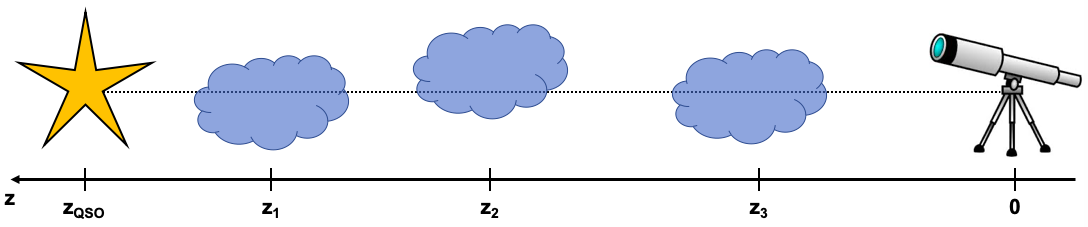
\includegraphics[scale=0.4]{schema_lya}
  \caption{bla}
  \label{fig:schema_lya}
\end{figure}
Un quasar, situé à un redshift $z_{QSO}$ émet de la lumière jusqu'à un observateur situé sur terre, à $z=0$. Trois absorbeurs sont disposés le long de la ligne de visée, à des redshifts $z_1$, $z_2$ et $z_3$. Ils représentent les structures à grande échelle de l'univers. L'hydrogène neutre et non excité qui constitue ces absorbeurs peut absorber les photons issus du quasar. Nous supposons que ces absorbeurs absorbent uniquement en \lya{} : les photons possédant une longueur d'onde $\lambda_{\mathrm{RF}} = \SI{1215.67}{\angstrom}$ dans le référentiel de l'absorbeur sont absorbés par l'hydrogène neutre, et leur électron effectuent une transition électronique de la couche $n=1$ à $n=2$. Plus l'absorbeur est dense, et plus le nombre de photons absorbés est important. Considérons à présent l'absorbeur 1. L'absorption \lya{} s'effectuant, sans son référentiel, à $\lambda_{\mathrm{RF}} = \SI{1215.67}{\angstrom}$, les photons absorbés sont ceux pour lesquels $\lambda_{QSO} = \num{1215.67} / (1+(z_{QSO} - z_{1})) \si{\angstrom}$ dans le référentiel du quasar. Depuis le référentiel de l'observateur, la raie \lya{} se trouve à $\lambda_{obs} = \num{1215.67} (1+z_{qso}) \si{\angstrom}$ et la raie d'absorption due à l'absorbeur 1 à $\lambda_{obs} = \num{1215.67} (1+z_{1}) \si{\angstrom}$.

\begin{itemize}
\item qso : $\lambda1 = 1215.67$ ; $\lambda2 = \frac{1215.67}{1 + z_{QSO} - z_{1}}$
\item abs1 : $\lambda1 = 1215.67 ( 1+ z_{QSO} - z_{1})$ ; $ \lambda2 = 1215.67$
\item obs : $\lambda1 = 1215.67 ( 1+z_{QSO})$ ; $\lambda2 = \frac{1215.67}{1 + z_{QSO} - z_{1}}(1+z_{QSO}) =? 1215.67(1+z_{1})$
\end{itemize}

% Supposons un  quasar, situé à un redshift $z_{qso}$. L'observateur est situé sur terre, à $z=0$. La raie \lya{}, dans le référentiel du quasar, possèdent une longueur d'onde $\lambda_{\mathrm{RF}} = \SI{1215.67}{\angstrom}$. Cependant, dans le référentiel de l'observateur, ils possèdent une longeur d'onde $\lambda_{obs} = \num{1215.67} (1+z_{qso}) \si{\angstrom}$. Sur leur trajet jusqu'à l'observateur, les photons émis par le quasar rencontrent les structures à grande échelle. Trois absorbeurs, aux redshifts $z_1$, $z_2$ et $z_3$, sont représentés. Supposons tout d'abord que ces structures sont faites uniquement d'hydrogène neutre non excité. Le premier absorbeur, au redshift $z_1$, peut absorber des photons issus du quasars. Les raies d'absorption possibles sont les raies de la série de Lyman, et la plus probable est l'absorption \lya{}. Ainsi, l'absorbeur 1 va absorber une partie des photons issus du quasar par absorption \lya{}, ces photons possèdent une longueur d'onde dans le référentiel de l'absorbeur 1 $\lambda_{\mathrm{RF-1}} = \num{1215.67} (1+(z_{qso} - z_1)) \si{\angtrom}$


\end{document}
